\documentclass[a4paper,onesided,12pt]{report}
\usepackage{styles/fbe_tez}
\usepackage[utf8x]{inputenc}
\renewcommand{\labelenumi}{(\roman{enumi})}
\usepackage{amsmath, amsthm, amssymb}
\usepackage[bottom]{footmisc}
\usepackage{cite}
\usepackage{graphicx}
\usepackage{longtable}
\graphicspath{{figures/}}
\usepackage{rotating}

\usepackage{multirow}
\usepackage{algorithm}
\usepackage{algorithmic}
\usepackage{floatpag}

\newtheorem{thm}{Theorem}[chapter]
\newtheorem{prop}[thm]{Proposition}
\newtheorem{lem}[thm]{Lemma}
\newtheorem{cor}[thm]{Corollary}
% COVER PAGE
\title{HIERARCHICAL MIXTURES OF GENERATORS IN GENERATIVE ADVERSARIAL NETWORKS}
\turkcebaslik{ÇEKİŞMELİ ÜRETİCİ AĞLARDA HİYERARŞİK ÜRETİCİ KARIŞIMLARI}
\degree{B.S., Computer Engineering, Boğaziçi University, 2017}
\author{Alper Ahmetoğlu}
\program{Computer Engineering}
\subyear{2019}

% APPROVED BY PAGE
\supervisor{Prof. Tunga Güngör}
\examineri{Assist. Prof. Emre Uğur}
\examinerii{Assist. Prof. Reyhan Aydoğan}
\dateofapproval{26.08.2019}

\begin{document}

\pagenumbering{roman}
\makemstitle % M.S. thesis
\makeapprovalpage
\begin{acknowledgements}
I want to thank Ethem Alpaydın for his guidance and his help through my undergraduate and graduate studies. I learned a lot from him in three years. Thanks to him, I very much enjoyed working on interesting problems.

I would like to thank Tunga Güngör, Emre Uğur, and Reyhan Aydoğan for accepting to be on my jury.

I am grateful to my family for their unconditional support. My first introduction to science would not be possible without them.

I thank Çağla Aksoy for her help, her patience, her presence, and her wholehearted support.

This thesis is partially supported by Boğaziçi University Research Funds with Grant Number 18A01P7.

The numerical calculations reported in this thesis were partially performed at TUBITAK ULAKBIM, High Performance and Grid Computing Center (TRUBA resources).
\end{acknowledgements}
\begin{abstract}
Recently proposed generative adversarial networks (GANs) are deep neural networks that are designed to model complex data distributions. The idea is to create a discriminator network that learns the borders of the data distribution; and a generator network which is trained to maximize the discriminator's loss to learn to generate samples from the data distribution. Instead of learning a global generator, one variant trains multiple generators, each responsible from one local mode of the data distribution. In this thesis, we review such approaches and propose the hierarchical mixture of generators, that learns a hierarchical division in a tree structure as well as the local generators in the leaves. Since these generators are combined softly, the whole model is continuous and can be trained using gradient-based optimization. Our experiments on five image data sets, namely, MNIST, FashionMNIST, CelebA, UTZap50K, and Oxford Flowers, show that our proposed model is as successful as the fully connected neural network. The learned hierarchical structure also allows for knowledge extraction.
\end{abstract}
\begin{ozet}
Çekişmeli üretici ağlar (ÇÜA), karmaşık veri dağılımlarını modellemek için öne sürülmüş derin sinir ağlarıdır. Ana düşünce, veri dağılımının sınırlarını öğrenen bir ayırıcı ağ üretip, bu ayırıcı ağ yardımı ile başka bir üretici ağı eğitmektir. Üretici ağ ayırıcı ağın hatasını yükseltmeye çalışarak örnekleme yapmayı öğrenir. Veri dağılımla-rında genelde birden fazla tepe bulunduğu için, ÇÜA'lar veri dağılımının hepsini öğren-mekte zorlanırlar. Evrensel tek bir üretici öğrenmek yerine, her biri dağılımın yerel bir kısmından sorumlu olan birden fazla üretici öğrenen varyantlar da bulunmaktadır. Bu tezde bu varyantları inceleyerek yeni bir mimari öne sürdük: hiyerarşik üretici karışımları. Bu mimaride ağaç, dağılımı hiyerarşik bir şekilde bölmeyi öğrenir; ağacın yapraklarında ise yerel üreticiler bulunmaktadır. Bu üreticiler esnek bir biçimde birleş-tirildiklerinden dolayı bütün model sürekli bir fonksiyondur ve türev bilgisine dayanan en iyileme metotları ile eğitilebilir. Beş farklı veri kümesinde (MNIST, FashionMNIST, CelebA, UTZap50K ve Oxford Flowers) yaptığımız deneyler göstermektedir ki öne sürdüğümüz mimari yoğun katmanlı sinir ağları kadar başarılıdır. Bunun dışında öğrenilen hiyerarşik yapı, veri dağılımı hakkında damıtılmış bir bilgi vermektedir.

\end{ozet}
\tableofcontents
\listoffigures
\listoftables
\begin{symbols}
\sym{$\mathbb{E}$}{Expectation}
\sym{$\|f\|_K$}{Function $f$ is $K$-Lipschitz}
\sym{$\mathcal{F}$}{Function family}
\sym{$I$}{Indicator function}
\sym{$\theta$}{Parameter set of the generator network}
\sym{$K$}{Kernel}
\sym{$\mathcal{N}(0, 1)$}{Normal distribution with mean 0 and variance 1.}
\sym{$\nabla_x f$}{Gradient of $f$ with respect to $x$}
\sym{$p(x)$}{Probability density function of random variable $x$}
\sym{$\mathbb{R}^d$}{Set of d-dimensional real numbers}
\sym{$p_{true}$}{Probability distribution of true samples}
\sym{$p_{fake}$}{Probability distribution of fake samples}
\sym{$W_1$}{1st Wasserstein distance}
\sym{$x$}{Real-valued vector}
\sym{$\|x\|_2$}{Euclidean norm of $x$}
\sym{$X$}{Data set}
\sym{$\phi$}{Parameter set of the discriminator network}

\end{symbols}

\begin{abbreviations}
 % Abbreviations in alphabetical order
\sym{AE}{Auto-encoder}
\sym{BiGAN}{Bidirectional Generative Adversarial Network}
\sym{C2ST}{Classifier Two-Sample Test}
\sym{CGAN}{Conditional Generative Adversarial Network}
\sym{DCGAN}{Deep Convolutional Generative Adversarial Network}
\sym{DNN}{Deep Neural Network}
\sym{EM}{Earth-Mover}
\sym{FID}{Fr\'echet Inception Distance}
\sym{GAN}{Generative Adversarial Network}
\sym{HME}{Hierarchical Mixture of Experts}
\sym{HME-GAN}{Hierarchical Mixture of Experts Generative Adversarial Network}
\sym{IS}{Inception Score}
\sym{JSD}{Jensen-Shannon Divergence}
\sym{KL}{Kullback-Leibler Divergence}
\sym{k-NN}{k-Nearest Neighbor}
\sym{LOO}{Leave One Out}
\sym{MAD-GAN}{Multi agent Diverse Generative Adversarial Network}
\sym{ME}{Mixture of Experts}
\sym{ME-GAN}{Mixture of Experts Generative Adversarial Network (ours)}
\sym{MEGAN}{Mixture of Experts Generative Adversarial Network}
\sym{MGAN}{Mixture Generative Adversarial Network}
\sym{PDF}{Probability Density Function}
\sym{ReLU}{Rectified Linear Unit}
\sym{SGD}{Stochastic Gradient Descent}
\sym{VAE}{Variational Auto-encoder}
\sym{WGAN}{Wasserstein Generative Adversarial Network}
\end{abbreviations}

\chapter{INTRODUCTION}
\label{chapter:intro}
\pagenumbering{arabic}

We are interested in the unsupervised problem of density estimation. That is, we are given a set of data points $X = \{x^{(i)} \in \mathbb{R}^d\}_{i=1}^N$ and assume that these are random events generated from some unknown probability density function (PDF) $p(x)$. Our aim is to approximate $p(x)$ with a proposal PDF $\hat{p}(x)$, using $X$. If we successfully approximate $p(x)$ with $\hat{p}(x)$, then we can use $\hat{p}(x)$ for later downstream tasks such as detecting the probability of an event, classification and generating new instances by sampling from $\hat{p}(x)$.

To be more concrete, we are in a search of a function $f(x)$ that mimics $p(x)$ using $X$. We further say that the true $f(x)$ should give the highest total probability for points in $X$. This is sometimes interpreted as ``the model that best explains the data'' and known as the \emph{maximum likelihood estimation}:
\begin{equation}
\underset{f \in \mathcal{F}}{\text{argmax}} \prod_{x^{(i)} \in X} f(x^{(i)})
\label{eq:mle}
\end{equation}
where $\mathcal{F}$ is the space of functions. We converted the problem into that of optimization. There are many optimization methods that can help us solve Equation \ref{eq:mle} analytically and/or approximately.

In the parametric case, we assume that $f(x)$ is a parametric model, for example, Gaussian distribution with mean $\mu$ and  covariance $\Sigma$. The problem then reduces to estimating $\mu$ and $\Sigma$, for example, maximum likelihood estimation. The other possibility is to assume that $f(x)$ can be modeled by a mixture of parametric distributions, for example, a mixture of Gaussians. Again, maximum likelihood estimation allows us to estimate the parameters of the component densities as well as their proportions. The third alternative is non-parametric estimation where we use the data points directly, and do not estimate parameters explicitly. We define \emph{kernels} that measures the distance of the queried point with its neighbors. For example, the kernel density estimator can be written as:
\begin{equation}
\hat{f}(x) = \frac{1}{nh} \sum_{i=1}^N K\left(\frac{x^{(i)}-x}{h}\right)
\label{eq:kde}
\end{equation}
where $K$ is the kernel function, and $h$ is called \emph{bandwidth}. $K$ and $h$ are the hyperparameters that define the shape of the fit. Each approach has its own advantages and disadvantages.
\begin{figure}[htbp]
\begin{center}
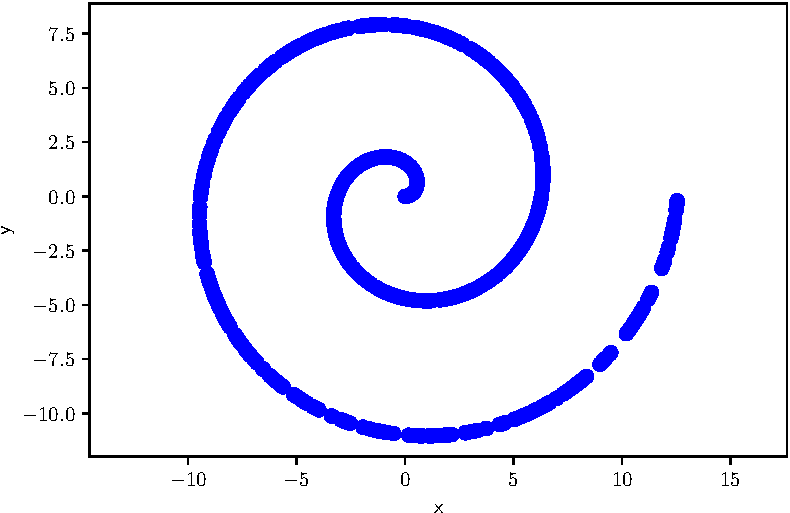
\includegraphics[width=0.5\columnwidth]{euc.pdf}
\end{center}
\caption[A spiral data set.]{A spiral data set. If we know $x_1=r*cos(r)$, $x_2=r*sin(r)$, the data become one-dimensional.}
\vskip\baselineskip
\label{fig:spiral}
\end{figure}

Another important point is the way the input is represented. For example in Figure \ref{fig:spiral}, if we use Cartesian coordinates, we probably fail, or find poor estimates for $p(x)$. If we know the transformation to polar coordinates, then we get a simpler problem. Both parametric models and non-parametric models will likely yield better results in polar coordinates for this specific problem. Therefore, the transformation is the golden nugget.

One of the advantages of \emph{deep neural networks} (DNNs) is that they can learn appropriate transformations in their hidden layers. Here, the transformation means that we map $X$ to $f_1(X; w_1)$, where $f_1$ denotes the computation that is done in the first layer of a DNN using weights $w_1$. In DNN, layers are organized serially:
\begin{equation}
\text{DNN}(X) = f_L (f_{L-1} ( \dots f_2( f_1(X; w_1); w_2); w_{L-1}); w_L)
\label{eq:dnn}
\end{equation}
where $f_i$ denotes the $i$th layer of the DNN with weights $w_i$. Earlier layers of a DNN learn basic primitives about $X$, and subsequent layers built more abstract transformations using primitive transformations. Such abstract representations lead to better \emph{generalization}, that is, they improve performance on unseen data \cite{bengio2009learning}. DNNs have achieved great success on a variety of real-world problems such as object recognition \cite{krizhevsky2012imagenet}, speech recognition \cite{hinton2012deep} and statistical machine translation \cite{sutskever2014sequence}.

In this thesis, we focus on a method known as \emph{generative adversarial networks} (GANs) \cite{goodfellow2014generative} for approximating densities with DNNs. We propose to use a hierarchical mixture of generators as the generative part of GAN. This helps alleviate the problem of mode collapse together with increased sample quality. Due to our hierarchical formulation, the learned representation can also be interpreted in a post-hoc way to see clusters in the data.

The rest of this work is organized as follows. Chapter \ref{chapter:gan} reviews the prerequisite knowledge about GANs. In Chapter \ref{chapter:multiple_gan}, we discuss previous works in literature that also use multiple generators. We explain our proposed model in detail in Chapter \ref{chapter:mixture_gan}. Our experimental results are given in Chapter \ref{chapter:exps}. We conclude and discuss future work in Chapter \ref{chapter:conc}.

\chapter{GENERATIVE ADVERSARIAL NETWORKS}
\label{chapter:gan}

\section{Introduction}
\label{sec:gan:intro}

The generative adversarial network (GAN) has been proposed to learn a generative model to model a data distribution, $p(x)$ \cite{goodfellow2014generative}. GAN is composed of two learners, a generator network $G$ and a discriminator network $D$. $G(z;\theta)$ learns to map $z$ sampled from an arbitrary distribution $p(z)$ to the target distribution $p(x)$. It is a trained model, generally a deep neural network, parameterized by $\theta$. The discriminator $D(x;\phi)$, another neural network with weights $\phi$, is trained to assign low scores to ``fake'' samples generated by $G(z;\theta)$ and high scores to samples from true $p(x)$ given in the training set. We do not show any true samples to $G$, instead train it to generate samples that will get high score from $D$ (see Figure \ref{fig:gan}). This is achieved with the following objective:
\begin{equation}
\label{eq:gan}
\underset{G}{\text{min}} \quad \underset{D}{\text{max}} \quad \mathbb{E}_{x \sim p(x)} [ \log{D(x;\phi)} ] + 
\mathbb{E}_{z \sim p(z)} [ \log{(1-D(G(z;\theta);\phi))} ]
\end{equation}
We optimize Equation \ref{eq:gan} by alternating between optimizing $D$ and $G$ with stochastic gradient descent (SGD) (pseudo-code is given in Figure \ref{alg:gan}). In the original paper  \cite{goodfellow2014generative}, it is shown that if $D$ and $G$ have enough capacity, this optimization minimizes the Jensen-Shannon divergence (JSD) between $p_{\text{true}}$ and $p_{\text{fake}}$, and therefore will converge to a point where $G$ exactly generates the target distribution $p(x)$. Note that we use a parametric family of functions defined by neural networks, and this might limit our functions' capacity and break the convergence guarantee. 
%
\begin{figure}[htbp]
\begin{center}
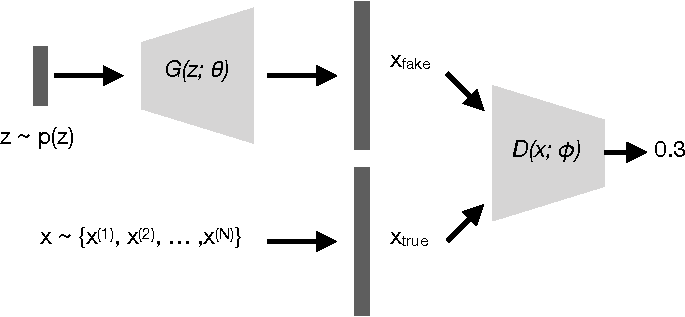
\includegraphics[width=0.75\textwidth]{gan.pdf}
\end{center}
\caption[GAN framework.]{GAN framework. Given an input $z$ that is drawn from $p(z)$, $G$ produces a \emph{fake} sample, $x_{fake}$. A \emph{real} sample $x_{real}$ that is drawn from the data set $X$ and $x_{fake}$ are given to $D$. $D$ is trained to classify $x_{fake}$ as 0 and $x_{real}$ as 1.}
\vskip\baselineskip
\label{fig:gan}
\end{figure}
%
\begin{figure}[htbp]
\begin{center}
\framebox[6.0in]{\begin{minipage}[t]{5.9in}
\begin{algorithmic}
\STATE
\STATE \textbf{Require:} Data set $X = \{x^{(i)}\}_{i=1}^N$, learning rate $\eta$.
\STATE Randomly initialize parameter sets $\theta$ of $G$ and $\phi$ of $D$;
\WHILE{stopping criterion satisfied}
\STATE Draw a batch of $m$ real samples $x_r \sim X$;
\STATE Draw a batch of $m$ noise vectors $z \sim \mathcal{N}(0, 1)$;
\STATE $x_f \Leftarrow G(z;\theta)$; \COMMENT{generated fake samples}
\STATE $\mathcal{L}_D \Leftarrow -\log D(x_r;\phi) - \log (1-D(x_f;\phi))$;
\STATE $\mathcal{L}_G \Leftarrow \log(1-D(x_f;\phi))$;
\STATE $\phi \Leftarrow \phi - \eta \nabla_{\phi} \mathcal{L}_D$; \COMMENT{update discriminator}
\STATE $\theta \Leftarrow \theta - \eta \nabla_{\theta} \mathcal{L}_G$; \COMMENT{update generator}
\ENDWHILE
\STATE
\end{algorithmic}
\end{minipage}}
\end{center}
\caption{The pseudo-code for training generative adversarial networks.}
\label{alg:gan}
\end{figure}

Once we learn a good $\theta$, $G$ can generate new data simply by sampling an input point $z$ and outputting $G(z;\theta)$. We can think of $G$ as a counterfeiter, who tries to produce \emph{fake} coins. On the other hand, $D$ is an inspector who tries to detect fake coins. When $D$ gets better at detecting fake coins, $G$ must produce coins that are of better quality to fool the inspector. This game will continue until $G$ finds a way to produce coins that exactly look like real ones. At that moment, $D$ is helpless, and can only make random guesses.

\section{Problems Related with GANs}
\label{sec:problems}

GANs are used successfully especially in image generation. A well-trained GAN can generate images that are almost indistinguishable by humans \cite{karras2017progressive,brock2018large,karras2019style}. Yet, there remain two main difficulties regarding the training: The first problem of mode collapse means that $G$ learns to generate some parts of $p(x)$ but not all; there are ways of being $x$ that cannot be generated for any $G(z)$. This is depicted in Figure \ref{fig:modecollapse}.

The second problem is of vanishing gradients. In order to optimize Equation \ref{eq:gan} for $G$, we should find gradients with respect to $\theta$. However $\nabla_{\theta} \log(1-D(G(z)))$ becomes zero in regions where $D$ is perfectly able to discriminate $p_{\text{true}}$ and $p_{\text{fake}}$. To remedy this, it is suggested to use a proxy loss, also known as non-saturating loss: $-\log D(G(z))$ \cite{fedus2017many}. This loss provides better gradients even when $D$ is optimal. However, it is shown that this loss no longer minimizes the JSD, but rather $KL(p_{\text{fake}} || p_{\text{true}}) - 2 JSD(p_{\text{fake}} || p_{\text{true}})$, where $KL$ is the Kullback-Leibler divergence \cite{arjovsky2017towards}. Moreover, they show that when $D$ gets better, the gradients of $G$ increase with an increasing variance. They conclude that this increasing variance might be the cause of the notorious instability of training GANs.

\begin{figure}[htbp]
\begin{center}
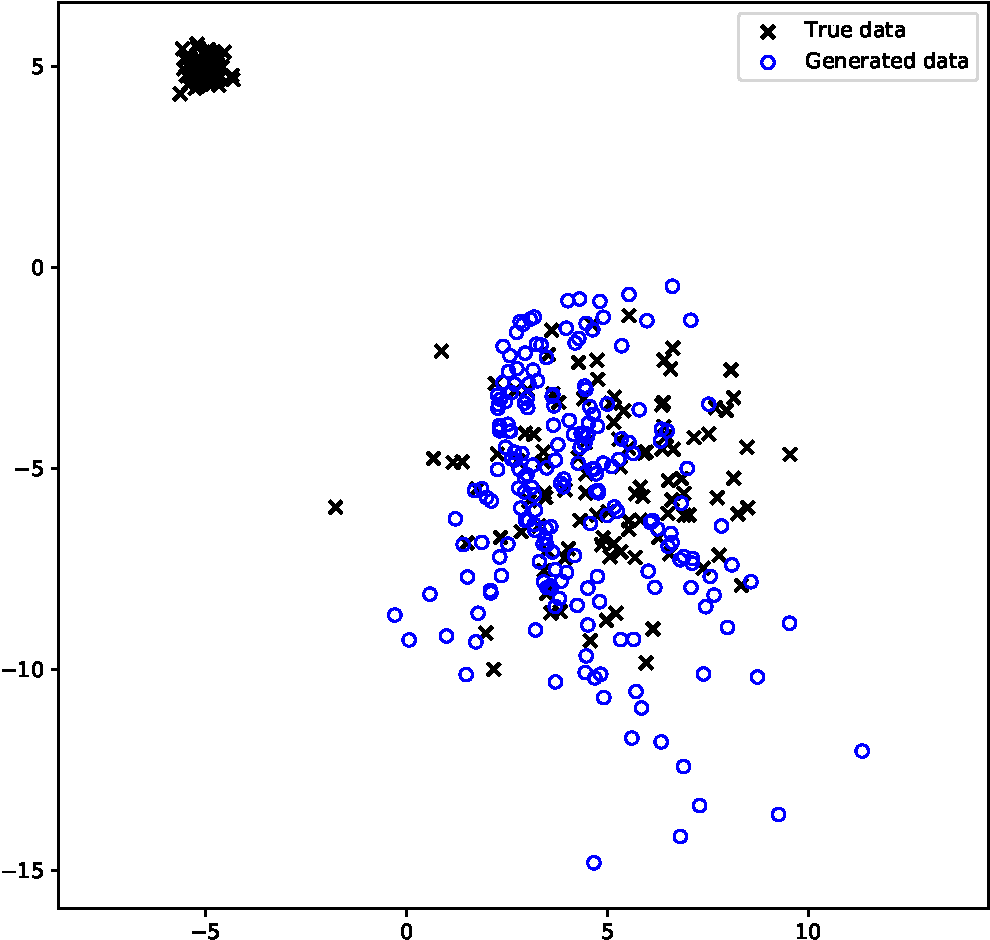
\includegraphics[width=0.9\textwidth]{modecollapse.pdf}
\end{center}
\caption[An example of a mode collapse]{An example of a mode collapse. The data set consists of samples from two Gaussian distributions, one on the top left with low variance and the other on the bottom right with high variance. The generator fails to model the one on the top left.}
\vskip\baselineskip
\label{fig:modecollapse}
\end{figure}

Recent work in the literature mainly focuses on these two problems. To solve problems related to training, researchers proposed either different GAN objectives \cite{arjovsky2017wasserstein,chen2016infogan,mao2017least,qi2017loss}, or regularization methods \cite{gulrajani2017improved,miyato2018spectral,radford2015unsupervised}, or architectures \cite{brock2018large,donahue2016adversarial,dumoulin2016adversarially,karras2017progressive,karras2019style,radford2015unsupervised,zhang2018self}. A good review can be found in \cite{creswell2018generative,hong2019generative,kurach2018gan}.

\section{Variants of GAN}
\label{sec:variants}

Before reviewing variants of GAN, we should first mention the variational auto-encoder (VAE) \cite{kingma2013auto} which also trains a generator but has a different network structure. A regular auto-encoder (AE) consists of an encoder network $E$ and a decoder network $D$. Given a data set $X=\{x^{(i)}\}_{i=1}^N$, AE minimizes the following:
\begin{equation}
\mathcal{L}_{rec} = \sum_{i=1}^N \frac{1}{2} \| x^{(i)} - D(E(x^{(i)};\phi);\theta) \|_2^2
\label{eq:recons}
\end{equation}
which is also known as the $\ell_2$ reconstruction loss. VAEs transform the idea to graphical models. They define the generative model as $p(z; \theta) p( x | z; \theta)$ and approximate the true posterior distribution $p(z|x)$ with a variational distribution $q(z|x;\phi)$. Here, $p(x | z; \theta)$ is the decoder and $q(z|x;\phi)$ is the encoder. A spherical Gaussian prior is assumed for $p(z)$. Two make computations easier, the variational distribution $q(z|x;\phi)$ is also chosen to be a multivariate Gaussian with diagonal covariance. Therefore, $q(z|x;\phi)$ outputs a mean and a standard deviation for each latent factor. To train the model, we simply minimize the reconstruction loss as in regular AE, and also minimize the KL divergence between $p(z)$ and $q(z|x;\phi)$ to approximate posterior. The reparameterization trick which they proposed \cite{kingma2013auto} should also be noted because it yields a gradient estimator which have lower variance then the na\"{i}ve Monte Carlo gradient estimator, which then helps us to train the variational model, $q(z|x;\phi)$. After training, we can simply draw $z$ from $p(z)$ and use the decoder network to produce $x$.

\begin{figure}[htbp]
\vskip\baselineskip
\begin{center}
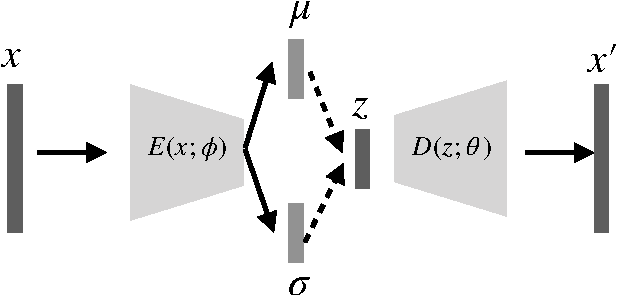
\includegraphics[width=0.8\textwidth]{vae.pdf}
\end{center}
\caption[Variational auto-encoder.]{Variational auto-encoder. Given $x$, $E$ outputs $\mu$ and $\sigma$ which defines a multivariate Gaussian. We sample $z$ from this Gaussian with reparameterization trick; $z = \sigma \odot \epsilon + \mu$ where $\epsilon \sim \mathcal{N}(0, 1)$. $D$ produces the output $x'$ given $z$.}
\vskip\baselineskip
\label{fig:vae}
\end{figure}

The conditional GAN (CGAN) \cite{mirza2014conditional} incorporates a label information $y$ to approximate class-conditional distribution $p(x|y)$. The extension is simple: We concatenate the one-hot label information $y$ to the noise vector $z$ and give it to $G$ as input. To get a conditioned gradient, we give $y$ together with $x$ as input to the $D$. Since $D$ learns the true class-conditional distribution $p(x|y)$, it pushes $G$ to approximate $p(x|y)$. After training, we can use $G$ to generate a sample from a specific class. We can embed more information in $y$, for example, in image-to-image translation, instead of class information we give a sketch of an image as $y$ and try to fill the image realistically \cite{isola2017image}. Given a real image (corresponds to $x$) and its sketch (corresponds to $y$), we ask $D$ whether this is a real example or not. Consequently, $G$ learns to create an image from its sketch. This is extended to translating from winter scenes to summer scenes, satellite views to map views, and so on. The same idea is also applied to super-resolution \cite{ledig2017photo} and image inpainting \cite{yeh2017semantic} where we choose the $(x, y)$ pairs accordingly. For example in super-resolution, $x$ is the high-resolution image and $y$ is its low-resolution version. The cycle GAN \cite{zhu2017unpaired} further extends the idea to also work with unpaired images by introducing a cycle-consistency loss. Apart from these extensions of CGAN, some methods incorporate the $y$ information in a better way than concatenating it with the input \cite{miyato2018cgans}.

In the original GAN, we learn a mapping from $p(z)$ to $p(x)$, but the reverse direction from $p(x)$ to $p(z)$ is not available. In the bidirectional GAN (BiGAN) \cite{donahue2016adversarial,dumoulin2016adversarially} there is an additional encoder $E$. $G$, as usual, generates a sample $G(z)$ given a noise vector $z$. $E$ generates a latent code $E(x)$ given a real sample $x$. Both $G$ and $E$ concatenate their input with their output producing pairs $(z, G(z))$ and $(E(x), x)$ respectively. The discriminator $D$ learns to discriminate between these two pairs. To maximize the loss of the discriminator, $G$ must produce vectors that look like $x$, likewise $E$ must produce vectors that look like $z$. When the training converges, these pairs $(z, G(z))$ and $(E(x), x)$ must be coherent with each other in order to maximize the loss of $D$. That is we expect $E(G(z))=z$  and $G(E(x))=x$ to hold.

There are many other ideas that are tried with GANs. The basic idea is the same: We train a DNN for problem $A$, which helps us to train another DNN for problem $B$, which in turn helps to learn $A$. Because they are trained in an iterative fashion, one can think that each DNN creates a curriculum for the other. For the case of GANs, $G$ first creates random noise. $D$ learns to discriminate the random noise and the training data, which is quite easy for high-dimensional data. With the help of $D$, $G$ starts to create better samples but not very good initially. The task gets iteratively harder for $D$ and likewise, when $D$ gets proficient, $G$ must learn finer details which is a harder task. There is a problem when the curriculum becomes unfair and the gradients vanish (or become unstable). In the next section, we review an approach to this problem, which we also use in our experiments.

\section{Wasserstein GAN}
\label{sec:wgan}
There are some shortcomings of the original GAN loss and its modified version, the non-saturating GAN loss. If $D$ becomes the optimal discriminator, then the gradients of $G$ vanish for the original loss. On the other hand, the non-saturating loss makes gradients unstable. One can think of training $D$ less, before we reach optimality, however there is no such principled way to control this optimality in the GAN framework \cite{arjovsky2017towards}.

Based on these observations, the Wasserstein GAN \cite{arjovsky2017wasserstein} is proposed. The motivation is to build a new distance measure that has good convergence properties even when the discriminator is optimal. They propose minimizing Earth-Mover (EM) distance, also known as 1st Wasserstein distance. The advantage is that Wasserstein distance is a convex function even when the supports of the two distributions do not intersect. It is defined as follows:
\begin{equation}
W_1(p_t, p_f) = \inf \quad \mathbb{E}_{(x,y) \sim (p_t, p_f)} [ \| x-y \| ]
\label{eq:emd}
\end{equation}
However, this formulation is known to be intractable. From the optimal transport view, this formulation tells us that the distance is the minimum one out of all transportation plans. Instead, we use the Kantorovich-Rubinstein duality, as in \cite{arjovsky2017wasserstein}:
\begin{equation}
W_1(p_t, p_f) = \underset{\|f\|_L \leq 1}{\sup} \mathbb{E}_{x\sim p_t} [f(x)] - \mathbb{E}_{x \sim p_f} [f(x)]
\label{eq:wd}
\end{equation}
where $\|f\|_L \leq 1$ implies 1-Lipschitz functions. Equation \ref{eq:wd} tells us that in order to find $W_1$ distance, we should find such $f$ that will maximize the difference. If there is no Lipschitz constraint, then we can find functions that will maximize the difference indefinitely. The Lipschitz constraint ensures that we are searching the function in a bounded region.

Now, to find the Wasserstein distance between two distributions, we can simply create a random neural network $f$ and maximize Equation \ref{eq:wd} with SGD. The function $f$ can be thought as a ``critic'' (instead of discriminator) since the output of the critic tells the generator how far it is from the true distribution. Then, for the generator, we minimize Equation \ref{eq:wd} since we know that doing so will bring two distributions closer. This formulation is called the Wasserstein GAN (WGAN) \cite{arjovsky2017wasserstein}.  The differences between WGAN and GAN are:
\begin{itemize}
	\item The discriminator outputs a real value, instead of a probability.
	\item The discriminator is constrained to be 1-Lipschitz.
	\item The discriminator should be trained till optimality (unlike GANs) since a better discriminator implies a better $W_1$ distance, and therefore better gradients to $G$.
\end{itemize}

The Lipschitz constraint is enforced through clipping weights of the critic function \cite{arjovsky2017wasserstein}. A follow-up work introduced a more principled way by applying gradient penalty to the critic \cite{gulrajani2017improved}.

The WGAN shows better convergence properties both in theory and in practice when compared with the original GAN. For this reason, we use the WGAN formulation with the gradient penalty \cite{gulrajani2017improved} in our experiments.

\section{Evaluation Metrics}
\label{sec:evaluation}

Another problem is of evaluating GANs. Unlike the Bayesian generative models where we can evaluate the quality of a model using the marginal likelihood (or with evidence lower bounds), there is no proper way of evaluating the GAN. The most frequently used measures are the Inception score (IS) \cite{salimans2016improved} and the Fr\'echet Inception distance (FID) \cite{heusel2017gans} since most of the papers include these scores. These two scores use Inception v3 network \cite{szegedy2016rethinking} that is pre-trained on ImageNet \cite{deng2009imagenet}.

\subsection{Inception Score}
\label{subsec:is}
In IS, the class-conditional distribution $p(y|x)$ is compared with the marginal class distribution $\int_x p(y|x) p(x)$. Here, probabilities are provided by the Inception network. The idea is that the entropy of $p(y|x)$ should be low if $x$ contains real-looking images since we believe Inception v3 is a good image classifier. On the other hand, the entropy of $\int_x p(y | x) p(x)$ should be high if the model outputs images that are not natural looking since no class will have high probability. The overall formulation is:
\begin{equation}
\label{eq:is}
\text{IS}=\exp (\mathbb{E}_{x \sim p_f} KL (p(y|x) || p(y))) 
\end{equation}

\subsection{Fr\'echet Inception Distance}
\label{subsec:fid}
In IS, we never look at the distribution of real images which is a problem. In FID, we take Inception network's activations in the layer before the last layer for both true samples and fake samples. These activations are then modeled with multivariate Gaussian distributions. Let us denote the mean and the covariance of true samples and fake samples as $(\mu_t, \Sigma_t)$ and $(\mu_f, \Sigma_f)$ respectively. Then, FID is calculated as follows:
\begin{equation}
\label{eq:fid}
\text{FID} = \| \mu_t - \mu_f \|_2^2 + \text{Tr}(\Sigma_t + \Sigma_f - 2(\Sigma_t \Sigma_f)^{1/2})
\end{equation}

\subsection{Nearest Neighbor Accuracy}
\label{subsec:nn}
In the classifier two-sample test (C2ST) \cite{lopez2016revisiting}, we train a classifier for two-class classification where classes are the true samples and the fake samples, then we use this classifier to assess whether the two distributions are close to each other. If these two distributions are very close to each other, the classifier cannot perform better than chance. In \cite{xu2018empirical}, they show that 1-nearest neighbor (1-NN) leave-one-out (LOO) classifier can detect mode collapse, mode drop, and sample diversity. The procedure is as follows. We take a set of real samples and fake samples. For each sample, we look at its nearest neighbor's label. This counts as the prediction of the model for the current sample. If the overall accuracy is around 50\%, we say these two distributions are very close to each other. Let us make the test only for real images and call this prediction accuracy metric 1-NN real. A higher 1-NN real accuracy implies samples that are near real samples are also real, therefore a mode drop. If this is very low, we can suspect that the generator overfits the target distribution. On the other hand, 1-NN fake accuracy assesses sample diversity. If 1-NN fake accuracy is high, then the samples are not diverse. 
Apart from this, human judgment is generally used by visualizing samples that are generated by the model to assess quality. Although this is not a good approach and only works for the image domain, we have no choice until we find a rigorous metric that can be trusted. An extensive review of evaluation methods can be found in \cite{borji2019pros}. In this study, we use FID and 5-NN accuracy as evaluation metrics where 5-NN accuracy is calculated with the same activations we calculate the FID score with. We also show a set of generated samples to let the reader decide the quality.


\chapter{COMBINING MULTIPLE GENERATORS IN GAN}
\label{chapter:multiple_gan}

The direction we pursue is to use multiple generators, each one responsible from a local region of the $p(z)$, and hence $p(x)$. Different local generators will learn to cover different modes and this will help alleviate the mode collapse problem. We review three previously proposed approaches that use a set of generators but in different ways.

\section{Multi Agent Diverse GAN}
\label{sec:madgan}

In the multi agent diverse GAN (MAD-GAN) \cite{ghosh2018multi}, there are multiple generators and each generator labels the fake data with its index. The discriminator not only separates true examples from fakes, but also learns the index of the generator for a fake. This additional classification problem forces generators to be local.

\begin{figure}[htbp]
\begin{center}
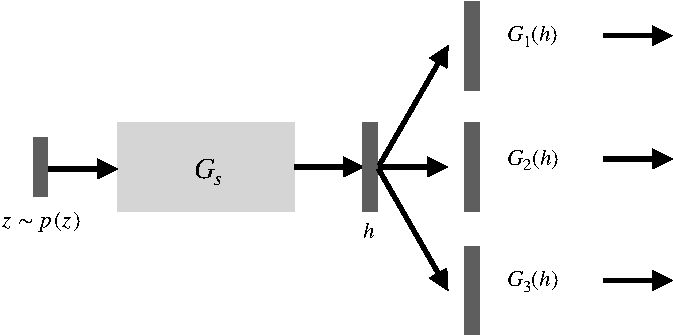
\includegraphics[width=0.75\columnwidth]{madgan.pdf}
\end{center}
\caption[Multi agent diverse GAN.]{Multi agent diverse GAN \cite{ghosh2018multi}. Given an input noise vector $z$, the shared network $G_s$ produces an intermediate representation $h$. From this representation, each generator $G_i$ outputs a sample.}
\vskip\baselineskip
\label{fig:models:madgan}
\end{figure}

The model is shown in Figure \ref{fig:models:madgan}. Given $z$, a shared neural network $G_s$ block produces $h$, an intermediate representation that is higher dimensional than $z$, which is used by a set of generators $\{G_i\}_{i=1}^K$. The discriminator is a $K+1$-class classifier with 0 for true, and $1$ to $K$ as the index of the generator for the fake instances. The discriminator should push the different generators to different modes to be able to solve the classification problem. More formally, the discriminator tries to minimize the following:
\begin{equation}
\min_{\phi} \quad -\mathbb{E}_{x \sim (p_t \cup p_f)} \left[ \sum_{j=0}^K r_j(x) \log D_j(x;\phi)\right]
\label{eq:madgan1}
\end{equation}
where $p_t$  and $p_f$ are the target and the fake distribution respectively, and $r$ is a one-hot vector with $K+1$ length. This is the regular cross-entropy error function. The cost function for the $i$th generator:
\begin{equation}
\min_{\theta} \quad \mathbb{E}_{z \sim p(z)} \log (1-D_0(G_i(z;\theta)))
\label{eq:madgan2}
\end{equation}
where $D_0$ represents the discriminator's probability output for real class.

Though there are multiple generators, we do not mix them in a cooperative manner. We also do not partition $p(z)$ and use each partition for different generators. This should rather be thought as each generator produces its interpretation of $p(z)$. Therefore, instead of partitioning $p(z)$ we introduce alternative generator functions for the same region in $p(z)$.
%
%
\section{Mixture GAN}
\label{sec:mgan}

The mixture GAN (MGAN) \cite{hoang2018mgan} is similar to MAD-GAN except that the classifer and the discriminator are separate. The discriminator is two-class as usual discriminating between true and fake examples, and there is a separate $K$-class classifier only for the fake examples.

\begin{figure}[htbp]
\begin{center}
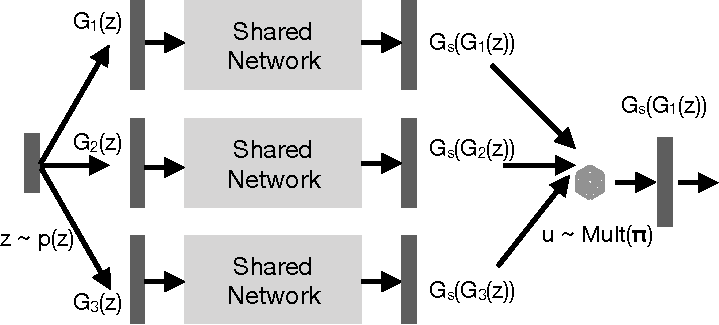
\includegraphics[width=0.75\columnwidth]{mgan.pdf}
\end{center}
\caption[Mixture GAN.]{Mixture GAN \cite{hoang2018mgan}. Each generator $G_i$ creates an abstract representation which is fed to the shared network $G_s$ to generate the output. One sample out of $K$ generated samples is selected at random and given to the discriminator.}
\vskip\baselineskip
\label{fig:models:mgan}
\end{figure}

The model is shown in Figure \ref{fig:models:mgan}. There is also the difference that the split of the generators is earlier. A set of generators $\{G_i\}_{i=1}^K$, transform $z$ and for all, the shared network $G_s$ produces the final output. A multinomial distribution is sampled to randomly select one of the generators. The parameters of the multinomial distribution are fixed. While the discriminator tries to discriminate between the fake and the real data as usual, the classifier tries to predict the index of the generator that produced the fake sample. These two networks share parameters treating the training of the discriminator/classifier as a multi-task learning problem.

\section{Mixtures of Experts GAN}
\label{sec:megan}

In the MEGAN \cite{park2018megan}, inspired from the mixtures of experts \cite{jacobs1991adaptive}, there is an additional gating model, which is also trained, that chooses among the different generators.

\begin{figure}[htbp]
\begin{center}
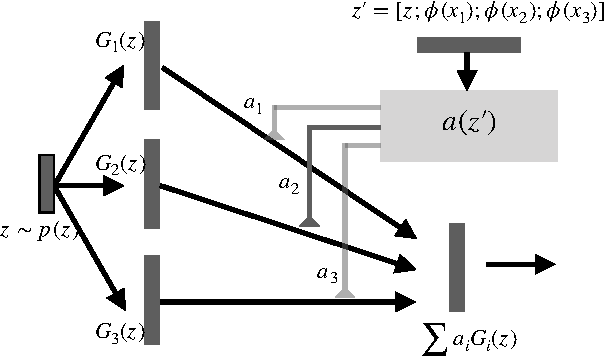
\includegraphics[width=0.75\columnwidth]{megan.pdf}
\end{center}
\caption[Mixture of experts GAN]{Mixture of experts GAN \cite{park2018megan}. Given $z$, each generator $G_i$ outputs a sample $x_i$. The gating network selects one generated sample among all based on $z$ and $\phi(x_i)$. $\phi$ returns the activation map of $x_i$ from earlier layers of $G_i$.}
\vskip\baselineskip
\label{fig:models:megan}
\end{figure}

The model is shown in Figure \ref{fig:models:megan}. There is a set of generators $\{G_i\}_{i=1}^{K}$ and an additional gating function, which takes as its input $z$ and some features from the generated $x$. Then Straight-Through Gumbel Softmax is applied which only selects one expert while allowing differentiability. The discriminator is still two-class. The gating model also has its parameters that are updated together with the generators. Although all generators generate an output, it is the gating model that decides which one is to be used. 

\vskip\baselineskip
Different from MAD-GAN and MGAN, in this approach $p(z)$ is partitioned into local parts. Since there is a gating network, each generator is only responsible for a local part of $p(z)$. However, this partitioning is rather hard since we only let one generator to be used. Also, the gating network takes features from the generators' outputs as its input, therefore the partitioning might be non-smooth.

%
\chapter{MIXTURES OF GENERATORS}
\label{chapter:mixture_gan}
All previous approaches use multiple generators yet these generators do not work cooperatively. We propose to use a mixture of generators that work cooperatively while also specializing in different regions of $p(z)$. We propose two different models: a flat mixture of generators and a hierarchical mixture of generators that are based on mixtures of experts (ME) \cite{jacobs1991adaptive} and hierarchical mixtures of experts (HME) \cite{jordan1994hierarchical} formulations, respectively. Unlike MEGAN which also uses the ME idea, we combine generators softly and use only the noise vector $z$ as the input.

\section{Flat Mixture of Generators}
\label{sec:me-gan}
The flat mixture of generators model, which we call ME-GAN (although the name is similar to MEGAN, we use the unmodified ME model unlike MEGAN, therefore keep the name with a dash), consists of local generators $\{G_i(z)\}_{i=1}^{K}$, and a gating function $a(z)$. The idea is that instead of learning a global generator, we divide the input space into regions and learn a set of local generators.
\begin{gather}
a_i(z) = \frac{\exp{(v_i z+v_{i_0})}}{\sum_{j=1}^K \exp{(v_j z+v_{j_0})}} \label{eq:me-gan1}\\
x = \sum_{i=1}^K a_i(z) G_i(z) \label{eq:me-gan2}
\end{gather}
For a given input $z$, the gating function outputs probabilities to decide how much to use each generator (Equation \ref{eq:me-gan1}). Because the gating function outputs a probability, we do not select just one generator but a convex combination of them (Equation \ref{eq:me-gan2}). For generators, we consider two options:
\begin{gather}
\text{Constant model:} \quad G_i(z) = c_i \label{eq:constant}\\
\text{Linear model:} \quad G_i(z) = W_i z + w_{i_0} \label{eq:linear}
\end{gather}
In the constant model (Equation \ref{eq:constant}), generators do not use the input but generate a constant vector response $c_i$. Although the generator response is constant, their combination weights $a$ are still dependent on the gating function and therefore depend on $z$. Because the combination of generators is convex, the set of possible outputs are constrained by the convex hull defined by $\{c_i\}_{i=1}^K$. The linear model (Equation \ref{eq:linear}) relaxes the job of the gating function by using a more general model. The error that is propagated through the discriminator, $\partial E / \partial x$, is distributed among generators with respect to their contribution (due to the chain rule), and each generator becomes responsible for modeling the input-output mapping in its region of expertise. In both formulations, the parameters of the gating function $\{v_i, v_{i_0}\}_{i=1}^K$ and the parameters of the generators $\{W_i, w_{i_0} \}_{i=1}^K$ (or $\{ c_i \}_{i=1}^K$ for constant model) are trained using SGD.

\section{Hierarchical Mixture of Generators}
\label{sec:hmgan}
Just like the hierarchical mixture of experts \cite{jordan1994hierarchical} go from the flat organization of mixture of experts  \cite{jacobs1991adaptive} to a tree, our proposed hierarchical mixture of generators (HME-GAN) go from a flat mixture of generators to a tree. HME-GAN and ME-GAN are the same except for the formulation of the gating functions. Let us think of a binary decision tree. The generators are at the leaves of this tree. At each internal node $m$ of the tree, there is a logistic function $\sigma_m(z)$ with parameters $\{v_m, v_{m_0}\}$:
\begin{equation}
\sigma_m(z) = \frac{1}{1+\exp{[-(v_m z + v_{m_0})]}}
\label{eq:sigmoid}
\end{equation}
Given an input $z$, this logistic function outputs a probability which serves as the mixture weights of the left and the right child. The response of an internal node $m$ can be written as:
\begin{equation}
x_m(z)=
	\begin{cases}
		\hfil G_m(z) &\text{if $m$ is a leaf} \\
		\hfil x_m^{L}(z) \sigma_m(z) + x_m^{R}(z)(1 - \sigma_m(z)) &\text{otherwise}
	\end{cases}
\label{eq:hmgan2}
\end{equation}
where $x_m^L$ and $x_m^R$ are the responses of the left and the right children, respectively. At each internal node $m$, we make a soft split and use $\sigma_m(z)$ of the response of the left tree and $1-\sigma_m(z)$ of the response of the right tree. This is carried out recursively until we arrive at the leaves where we have the generator responses, $G_i(z)$. Again, we are taking a convex combination of the generator responses. In ME-GAN, the $i$th generator is mixed with the weight:
\begin{equation}
a_i(z) = \frac{\exp{(v_i z + v_{i_0})}}{\sum_{j=1}^K \exp{(v_j z + v_{j_0})}}
\label{eq:fm_mix}
\end{equation}
whereas in HME-GAN, this is:
\begin{gather}\label{eq:hm_mix}
a_i(z) = \prod_{j \in Pred(i)} \sigma_j^{\delta_1^{(j)}}(z) (1-\sigma_j(z))^{\delta_2^{(j)}}\\
(\delta_1^{(j)}, \delta_2^{(j)}) =
	\begin{cases}
		(1, 0) & \text{if $i$ lies in the left subtree of $j$} \\
		(0, 1) & \text{otherwise}	
	\end{cases}
\end{gather}
where $Pred(i)$ is the predecessors of the leaf $i$. This model is differentiable, too, which lets us learn the set of parameters (in the gating nodes and the generators at the leaves) with SGD.

\chapter{EXPERIMENTS}
\label{chapter:exps}

\section{Data Sets}
\label{sec:datasets}
We test and compare our proposed mixture models ME-GAN and HME-GAN with related models, namely, MADGAN, MGAN, and MEGAN, on five image data sets that are widely used in GAN literature: MNIST \cite{lecun1998gradient}, FashionMNIST \cite{xiao2017fashion}, CelebA \cite{liu2015deep},  UTZap50K \cite{yu2014fine}, and Oxford Flowers (which we shorten as ``Flowers'') \cite{nilsback2008automated}.

MNIST is a data set that contains gray-scale handwritten digits of size $28 \times 28$ pixels. There are 60,000 training samples and 10,000 test samples. FashionMNIST is a data set of fashion products such as t-shirts, trousers, sneakers. It is inspired from MNIST and has the same image size with the same number of examples. It is designed to be a drop-in replacement from MNIST and known to be a harder baseline. For these two data sets, we resize the images to $32 \times 32$ pixels, to be able to use the same kind of deconvolutional architecture repeatedly. We use all the 10,000 examples in the test set for evaluation.

CelebA contains celebrity faces with 40 different annotated labels. There are 10,177 distinct people with a total of 202,599 images in color. We use the aligned-and-cropped version of the data set. There is no separate test set. We randomly select 10,000 test images and use them only for evaluation. These images contain very different backgrounds so we center-crop an area of $148 \times 148$ and then resize it to $64 \times 64$ pixels.

UTZap50K is a shoe data set of 50,000 catalog images in color. There are four major categories with many subcategories as brand names. We resize all images to $64 \times 64$. We randomly select 5,000 test images and use them only for evaluation.

Oxford flowers is a flower data set with 102 different categories with a total of 8198 images in color. There are around 80 images per class. We resize all images to $64 \times 64$. We use 1,000 test images for evaluation.

\begin{figure}[htbp]
\begin{center}
	\begin{tabular}{c}
		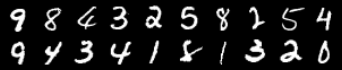
\includegraphics[width=0.85\linewidth]{mnist_dataset.png} \\
		{\footnotesize (a) MNIST} \\
		\vspace{0cm}\\
		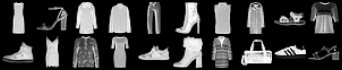
\includegraphics[width=0.85\linewidth]{fashion_dataset.png} \\
		{\footnotesize (b) FashionMNIST} \\
		\vspace{0cm}\\
		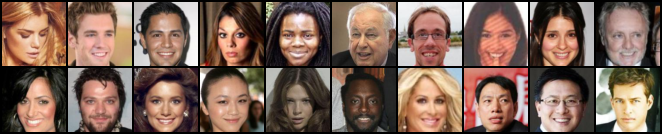
\includegraphics[width=0.85\linewidth]{celeba_dataset.png} \\
		{\footnotesize (c) CelebA} \\
		\vspace{0cm}\\
		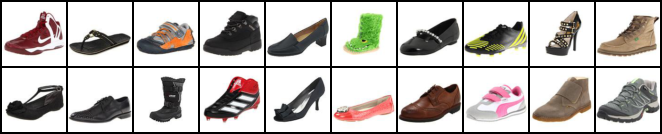
\includegraphics[width=0.85\linewidth]{utzap50k_dataset.png} \\
		{\footnotesize (d) UTZap50K} \\
		\vspace{0cm}\\
		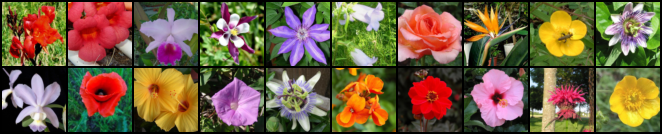
\includegraphics[width=0.85\linewidth]{flowers_dataset.png} \\
		{\footnotesize (e) Oxford Flowers}
	\end{tabular}
\end{center}
\caption{Random examples from the five data sets used in this work.}
\vskip\baselineskip
\label{fig:datasets}
\end{figure}

Some examples from each data set are shown in Figure \ref{fig:datasets}. All images contain pixel intensities in the range $[0, 255]$, which we normalized to range $[-1, 1]$. For MNIST and FashionMNIST, there are $32 \times 32=1024$ input features. The other three data sets are in color have three channels for red, green, blue pixel intensities; they hence have 64 $\times$ 64 $\times$ 3 $=$ 12,288 input features. 

\section{Experimental Setup}
\label{sec:setup}

\subsection{The Convolutional Pipeline}
\label{subsec:conv}

Our experiments are done in the image domain. It is known that using a convolutional architecture for tasks that involve images increases performance dramatically. For example, although the set of human face images contain many modes, textures are quite the same. For this reason, we incorporate transposed convolutional (also known as deconvolutional) layers in both of our models. Instead of generating samples directly in the data domain $x$, our mixture models first generate an abstract representation $h$, which is given to a transposed convolutional architecture $G_s$. This architecture then produces the output $x$. For the human face example, local generators create an abstract representation and $G_s$ produces the actual image given this abstract representation. For other domains where data points share common features, another domain specific architecture can be used to increase the performance given that the architecture is differentiable. The pipelines for ME-GAN and HME-GAN are depicted in Figure \ref{fig:models:me-gan} and \ref{fig:models:hmegan} respectively. Note that it is only $G$ that is modeled with ME or HME, $D$ remains the usual deep convolutional neural network.

\begin{figure}[htbp]
\begin{center}
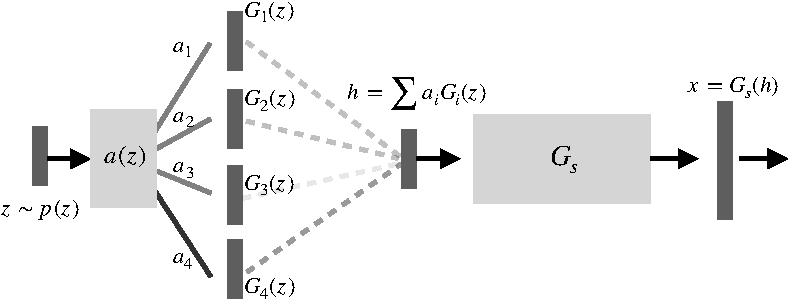
\includegraphics[width=0.98\columnwidth]{me-gan.pdf}
\end{center}
\caption[ME-GAN model]{ME-GAN model. Given $z$, each $G_i$ outputs a latent representation. These representations are mixed with weights $a_i$ which are provided by the gating function. The shared network $G_s$ produces the final output.}
\vskip\baselineskip
\label{fig:models:me-gan}
\end{figure}

\begin{figure}[htbp]
\begin{center}
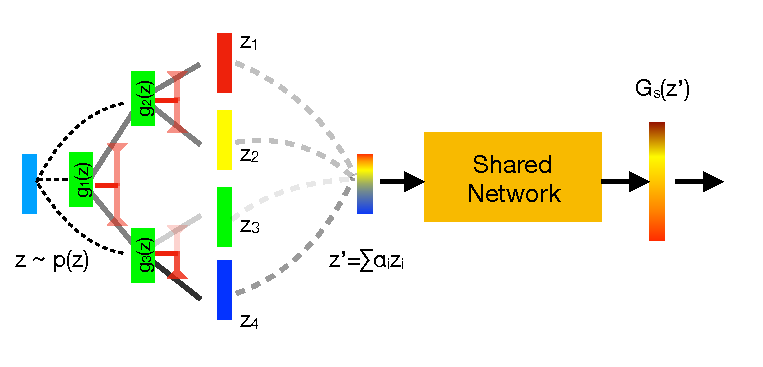
\includegraphics[width=0.98\columnwidth]{hmegan.pdf}
\end{center}
\caption[HME-GAN model]{HME-GAN model. Each $G_i$ creates a latent representation from $z$ as in ME-GAN. However, each $a_i$ is calculated by multiplying the $\sigma$ values along the path from the leaf to the root (Equation \ref{eq:hm_mix}). As in ME-GAN, $a_i$ values sum up to one.}
\vskip\baselineskip
\label{fig:models:hmegan}
\end{figure}


\subsection{Network Architectures}
\label{subsec:architecture}
The following settings are used in all experiments unless otherwise stated. We introduce multiple generators at the earlier levels of the model, and use a parameter-shared convolutional network on top of multiple generators as shown in Figures \ref{fig:models:me-gan} and \ref{fig:models:hmegan}. The discriminator part is the same for all models except MADGAN and MGAN. In MADGAN, the last layer of the discriminator contains $K+1$ units, instead of one. In MGAN, the last layer contains two parallel fully-connected layers, one of which outputs $K$ units for predicting the index of the generator and the other one outputs a probability for real \emph{vs.} fake classification. The convolutional architecture that we use for both the discriminator and the generator is the deep convolutional GAN (DCGAN) \cite{radford2015unsupervised}. MNIST and FashionMNIST are $32\times 32$ pixels and other data sets are $64\times 64$ pixels, the architectures used for two cases are given in Tables \ref{tab:smallmodel} and \ref{tab:largemodel}. The layers two to five are convolutional (or transposed convolutional) layers. First layer is a fully-connected (FC) layer for the baseline model, an ME layer for MEGAN and ME-GAN, and an HME layer for HME-GAN. For MADGAN and MGAN, this layer contains multiple fully-connected layers. The dimensionality of the input $z$ is set to 100. For the non-linearity, we used the rectified linear unit (ReLU) in the hidden layers. We did not use any normalization in $G$ but used layer normalization \cite{lei2016layer} in $D$ for ME-GAN and HME-GAN. We employed batch normalization both in $G$ and in $D$ for MADGAN, MGAN, and MEGAN.

\begin{table}[thbp]
\vskip\baselineskip
\caption[The generator and the discriminator networks for $32 \times 32$ sized data sets.]{The generator and the discriminator networks that are used with MNIST and FashionMNIST, which have $32\times 32$ gray-scale images. For convolutional layers, kernel size is set to $4 \times 4$ with a stride of $2 \times 2$ and with a padding of 1.}
\vskip\baselineskip
\begin{center}
\begin{tabular}{|l|c|c|c|c|}
\hline
\multicolumn{5}{|c|}{Generator Network}\\
\hline
Layer & In Channels & In Resolution & Out Channels & Out Resolution \\
\hline
Fully-Conn. & 100 & $1 \times 1$ & 256 & $4 \times 4$\\
\hline
Transp. Conv. & 256 & $4 \times 4$ & 128 & $8 \times 8$\\
\hline
Transp. Conv. & 128 & $8 \times 8$ & 64 & $16 \times 16$\\
\hline
Transp. Conv. & 64 & $16 \times 16$ & 1 & $32 \times 32$\\
\hline
\multicolumn{5}{|c|}{Discriminator Network}\\
\hline
Layer & In Channels & In Resolution & Out Channels & Out Resolution \\
\hline
Conv. & 1 & $32 \times 32$ & 64 & $16 \times 16$\\
\hline
Conv. & 64 & $16 \times 16$ & 128 & $8 \times 8$\\
\hline
Conv. & 128 & $8 \times 8$ & 256 & $4 \times 4$\\
\hline
Fully-Conn. & 256 & $4 \times 4$ & 1 & $1 \times 1$\\
\hline
\end{tabular}
\label{tab:smallmodel}
\end{center}
\end{table}

\begin{table}[thbp]
\vskip\baselineskip
\caption[The generator and the discriminator networks for $64 \times 64$ sized data sets.]{The generator and the discriminator networks that are used with CelebA, UTZap50K, and Oxford Flowers which are $64\times 64$ images in color. For convolutional layers, kernel size is set to $4 \times 4$ with a stride of $2 \times 2$ and with a padding of 1.}
\vskip\baselineskip
\begin{center}
\begin{tabular}{|l|c|c|c|c|}
\hline
\multicolumn{5}{|c|}{Generator Network}\\
\hline
Layer & In Channels & In Resolution & Out Channels & Out Resolution \\
\hline
Fully-Conn. & 100 & $1 \times 1$ & 512 & $4 \times 4$\\
\hline
Transp. Conv. & 512 & $4 \times 4$ & 256 & $8 \times 8$\\
\hline
Transp. Conv. & 256 & $8 \times 8$ & 128 & $16 \times 16$\\
\hline
Transp. Conv. & 128 & $16 \times 16$ & 64 & $32 \times 32$\\
\hline
Transp. Conv. & 64 & $32 \times 32$ & 1 & $64 \times 64$\\
\hline
\multicolumn{5}{|c|}{Discriminator Network}\\
\hline
Layer & In Channels & In Resolution & Out Channels & Out Resolution \\
\hline
Conv. & 1 & $64 \times 64$ & 64 & $32 \times 32$\\
\hline
Conv. & 64 & $32 \times 32$ & 128 & $16 \times 16$\\
\hline
Conv. & 128 & $16 \times 16$ & 256 & $8 \times 8$\\
\hline
Conv. & 256 & $8 \times 8$ & 512 & $4 \times 4$\\
\hline
Fully-Conn. & 512 & $4 \times 4$ & 1 & $1 \times 1$\\
\hline
\end{tabular}
\label{tab:largemodel}
\end{center}
\end{table}

\subsection{Hyperparameters}
\label{subsec:hyperparameter}
For ME-GAN and HME-GAN, the Wasserstein loss \cite{arjovsky2017wasserstein} with gradient penalty \cite{gulrajani2017improved} is used. We adopted the suggested hyperparameter setting for Wasserstein loss recommended in \cite{gulrajani2017improved}, namely two-sided gradient penalty with a constant of $10.0$. The discriminator is trained five times per optimization step of the generator. We cannot find a trivial way of using Wasserstein loss for MADGAN and MGAN since these methods make multi-class classification. We experimented Wasserstein loss on MEGAN but it did not give good results in our setting. Therefore, we use the vanilla log-likelihood GAN loss (the non-saturating version) for MADGAN, MGAN, and MEGAN. We used Adam optimizer \cite{kingma2014adam} with amsgrad option \cite{reddi2019convergence}. The learning rate is set to $0.0001$ with beta values of Adam set to $(0.5, 0.999)$. The batch size is set to 128.

\subsection{Evaluation}
\label{subsec:eval}
For the evaluation of GAN methods, we used the most popular evaluation criteria that are the Fr\'echet Inception distance (FID) \cite{heusel2017gans} and the two-sample test (C2ST) \cite{lopez2016revisiting}, here, 5-nearest neighbor (5-NN) leave-one-out accuracy. Both FID and 5-NN accuracy are calculated with the activations before the softmax layer (2048-dim) of Inception v3 \cite{szegedy2016rethinking}. Lower FID scores are better and 5-NN accuracies that are close to 50\% are better. All models are run five times with different random seeds, and we report the mean and standard deviations.

The seed numbers are set to {2019, 2020, 2021, 2022, 2023} for five different runs. Except for CuDNN \cite{chetlur2014cudnn} operations which are not deterministic but do not affect experiment results, all experiments are reproducible with given seeds. PyTorch auto-differentiation library \cite{paszke2017automatic} is used to automatically calculate gradients by exploiting the chain rule of Calculus.

\section{A Toy Example}
\label{sec:toy}
First, for the sake of the understanding of the model, we made a toy experiment (Figure \ref{fig:toy}). We are given a spiral-like shaped two-dimensional data set. We trained an HME-GAN model with a depth of three, so there are eight generators at the leaves. At the top level, we see the trained model's response. The input noise vector is drawn from a one-dimensional Gaussian distribution with zero mean and unit variance. The possible input range is shown with colors on the top box in Figure \ref{fig:toy}. The output of the model is also colored, indicating which part of the input maps to which part of the output. We visualized each node's responsibility by softly counting the gating values. On the first level of the tree, we see that the overall output of the model is divided into two, the left responsible for the inner region, and the right responsible for the outer region. When we go down in the tree, the responsibility is distributed among children. At the final level, where the leaves are located, there are generator functions. Notice that each generator is used in a local region. We also see that some generators are not used at all.

This example shows that even when the distribution is very non-linear, we can model it with simple linear models by hierarchically combining them. The hierarchical combination dissects the problem into two at each level, easing the problem in a divide-and-conquer fashion.

\begin{figure}[htbp]
\begin{center}
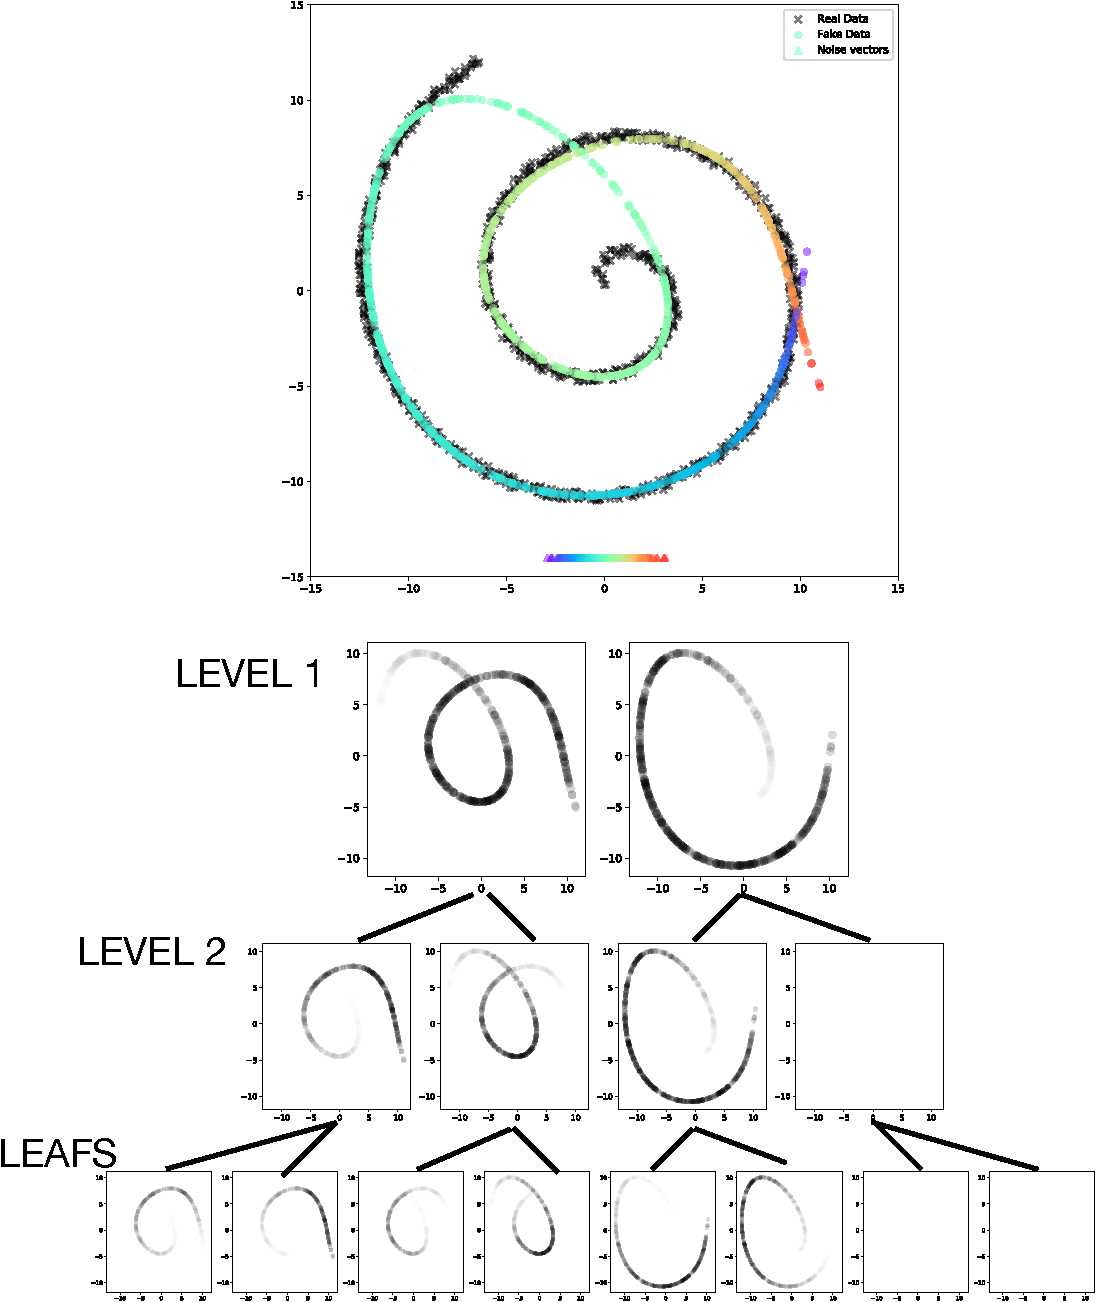
\includegraphics[width=0.9\textwidth]{toy.pdf}
\end{center}
\caption[The average responses of tree nodes of HME-GAN on a spiral data set.]{The average responses of tree nodes of HME-GAN on a spiral data set. The data set is represented with black crosses. The output of the model is colored dots. These colors represent different regions of the input.}
\vskip\baselineskip
\label{fig:toy}
\end{figure}

\section{Flat Mixture vs. Hierarchical Mixture}
We have shown two different ways of combining multiple generators, namely, the flat mixture and the hierarchical mixture. Now, we want to see whether there is a qualitative difference between these two models. We use trees of different depths, and we also test a flat mixture of generators with the equal number of leaves. For example, we have a tree of depth five with 32 leaves and a flat mixture of 32 leaves. In the former case, for each leaf, we have five binary gatings; in the latter case, there is one gating that chooses one of 32. For the hierarchical model, we tested trees with depths from five to eight. To get the same number of leaves, we used 32, 64, 128 and 256 generator experts in the flat mixture.

\begin{figure}[htbp]
\begin{center}
\begin{tabular}{c}
	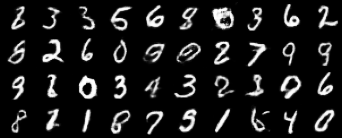
\includegraphics[width=0.75\linewidth]{me_samples_mnist.png} \\
	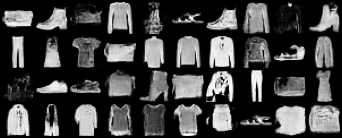
\includegraphics[width=0.75\linewidth]{me_samples_fashion.png}
\end{tabular}
\end{center}
\caption{Samples generated using ME-64 on $32 \times 32$ sized data sets.}
\vskip\baselineskip
\label{fig:samples_me}
\end{figure}

\begin{figure}[htbp]
\begin{center}
	\begin{tabular}{c}
		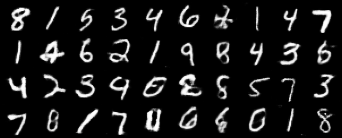
\includegraphics[width=0.75\linewidth]{hme_samples_mnist.png} \\
		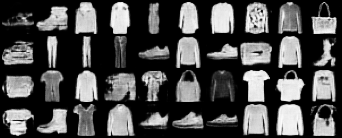
\includegraphics[width=0.75\linewidth]{hme_samples_fashion.png}
	\end{tabular}
\end{center}
\caption{Samples generated using HME-6 on $32 \times 32$ sized data sets.}
\vskip\baselineskip
\label{fig:samples_hme}
\end{figure}

\begin{figure}[htbp]
\begin{center}
	\begin{tabular}{c}
		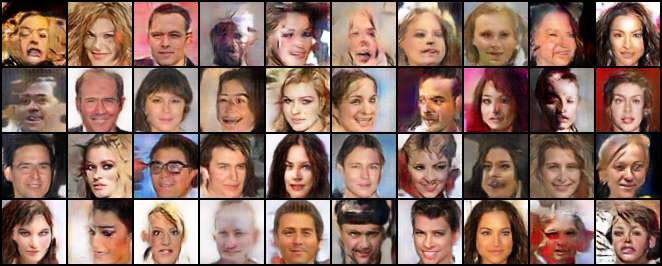
\includegraphics[width=0.9\linewidth]{me_samples_celeb.png} \\
		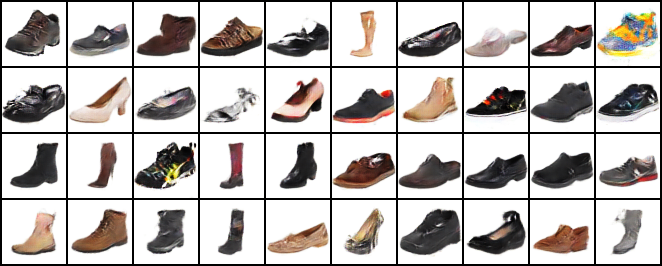
\includegraphics[width=0.9\linewidth]{me_samples_utzap50k.png} \\
		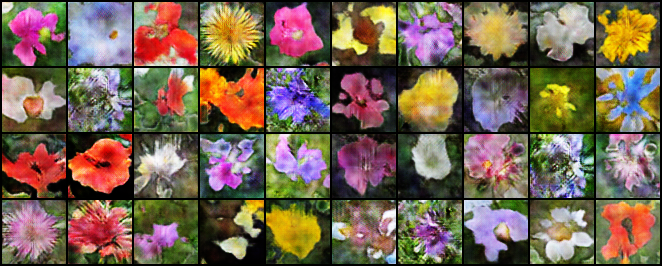
\includegraphics[width=0.9\linewidth]{me_samples_flowers.png}
	\end{tabular}
\end{center}
\caption{Samples generated using ME-64 on $64 \times 64$ sized data sets.}
\vskip\baselineskip
\label{fig:samples_me2}
\end{figure}

\begin{figure}[htbp]
\begin{center}
	\begin{tabular}{c}
		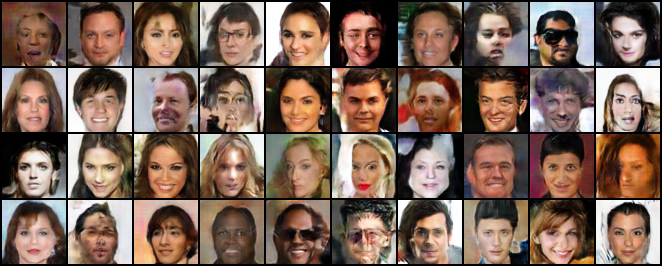
\includegraphics[width=0.9\linewidth]{hme_samples_celeb.png} \\
		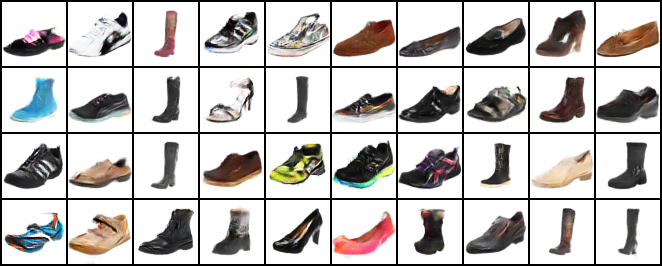
\includegraphics[width=0.9\linewidth]{hme_samples_utzap50k.png} \\
		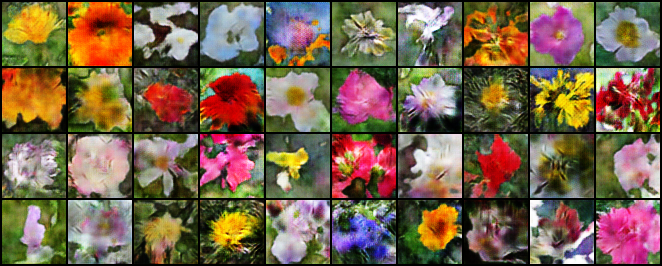
\includegraphics[width=0.9\linewidth]{hme_samples_flowers.png}
	\end{tabular}
\end{center}
\caption{Samples generated using HME-6 on $64 \times 64$ sized data sets.}
\vskip\baselineskip
\label{fig:samples_hme2}
\end{figure}

Some samples generated from ME-64 and HME-6 are shown in Figures \ref{fig:samples_me} to \ref{fig:samples_hme2} for visual inspection. It can be seen that these are quite realistic and contain diversity for both models. We also visualized the average generator responses of ME and HME for FashionMNIST data set in Figure \ref{fig:leaves}. To calculate this, we count the gating values of leaves for each generated image. Then, for each leaf, we take a weighted average of generated images where weights are gating values of a leaf for each image. This will give us a leaf's average response. We can see from the figure that the HME leaves are more diverse and local when compared with ME leaves. However, this figure is not about sample quality or sample diversity. It is rather about the relation of leaves with each other. Leaves of the ME model seem more blurry. This says that leaves of ME are not specialized in a region of $p(z)$ but rather used throughout in many regions of $p(z)$. To understand this clearly, we also show the covariance matrices of leaf gating values in Figure \ref{fig:covariances}. These are $64 \times 64$ matrices where each index corresponds to a leaf. For example, for both matrices, we see that the diagonal values are higher than others. This implies leaves are rather used alone, or used with high proportion. For ME, correlations are randomly scattered. Its counterpart HME has correlations gathered around the diagonal. Furthermore, we can see spectral squares of sizes $4 \times 4$ and $8 \times 8$. This shows that cooperations are done in a hierarchical way.

\begin{figure}[htbp]
\begin{center}
	\begin{tabular}{c}
		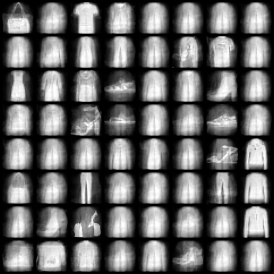
\includegraphics[width=0.55\linewidth]{me_leaves_fashion.png} \\
		{\footnotesize (a) ME-64} \\
		\vspace{0cm} \\
		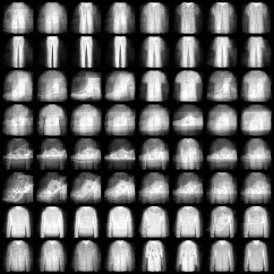
\includegraphics[width=0.55\linewidth]{hme_leaves_fashion.png} \\
		{\footnotesize (b) HME-6}
	\end{tabular}
\end{center}
\caption[The average responses of generators at the leaves for ME-64 and HME-6.]{The average responses of generators at the leaves for ME-64 and HME-6. We see that HME-6 responses are more localized compared to ME-64.}
\vskip\baselineskip
\label{fig:leaves}
\end{figure}

\begin{figure}[htbp]
\begin{center}
	\begin{tabular}{c}
		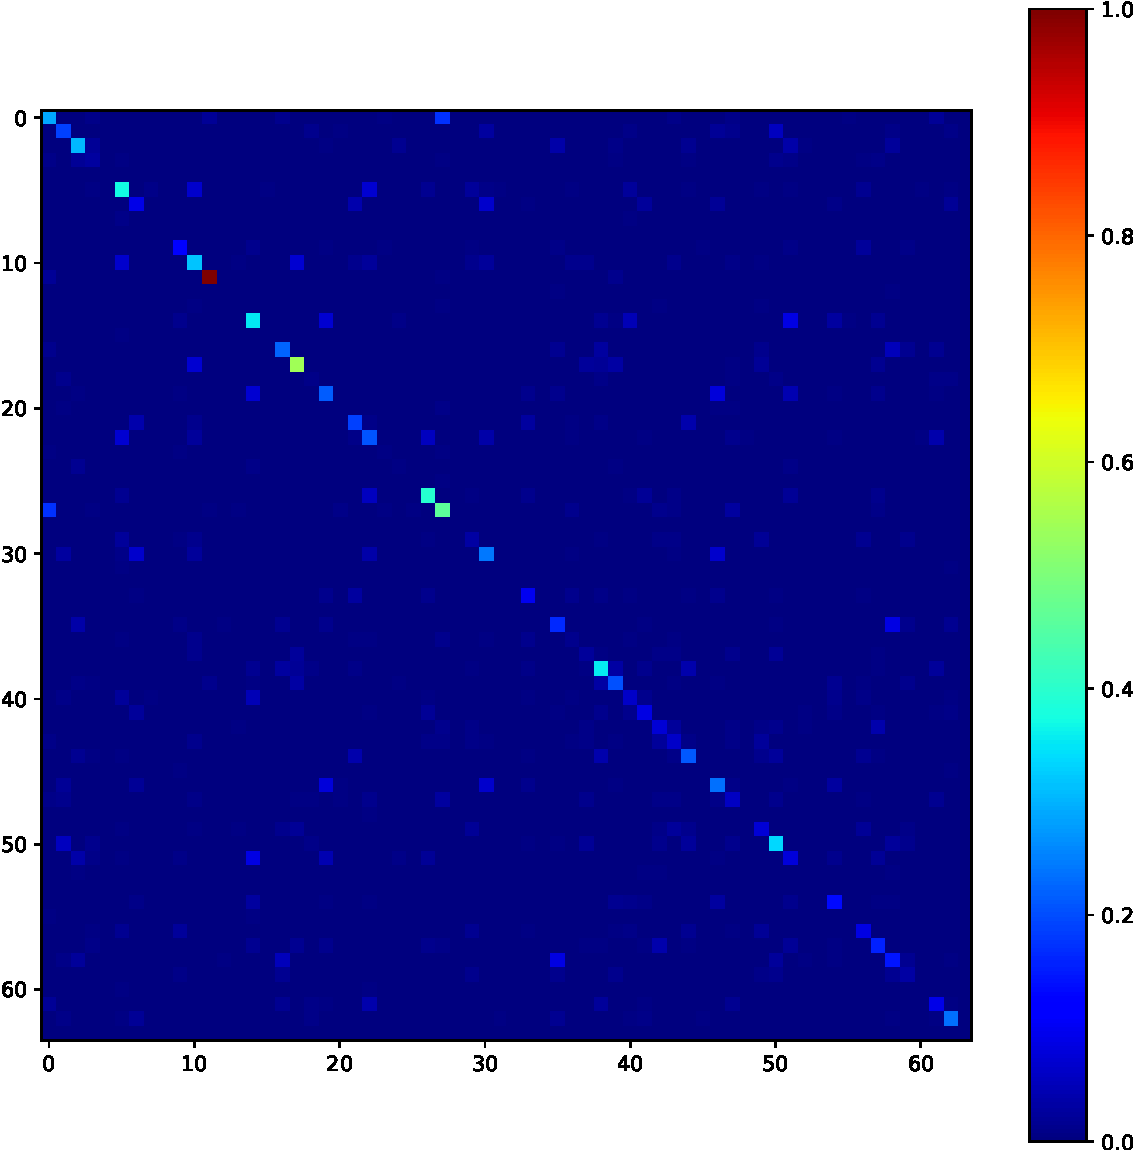
\includegraphics[width=0.5\linewidth]{cov_me.pdf} \\
		{\footnotesize (a) ME-64} \\
		\vspace{0cm} \\
		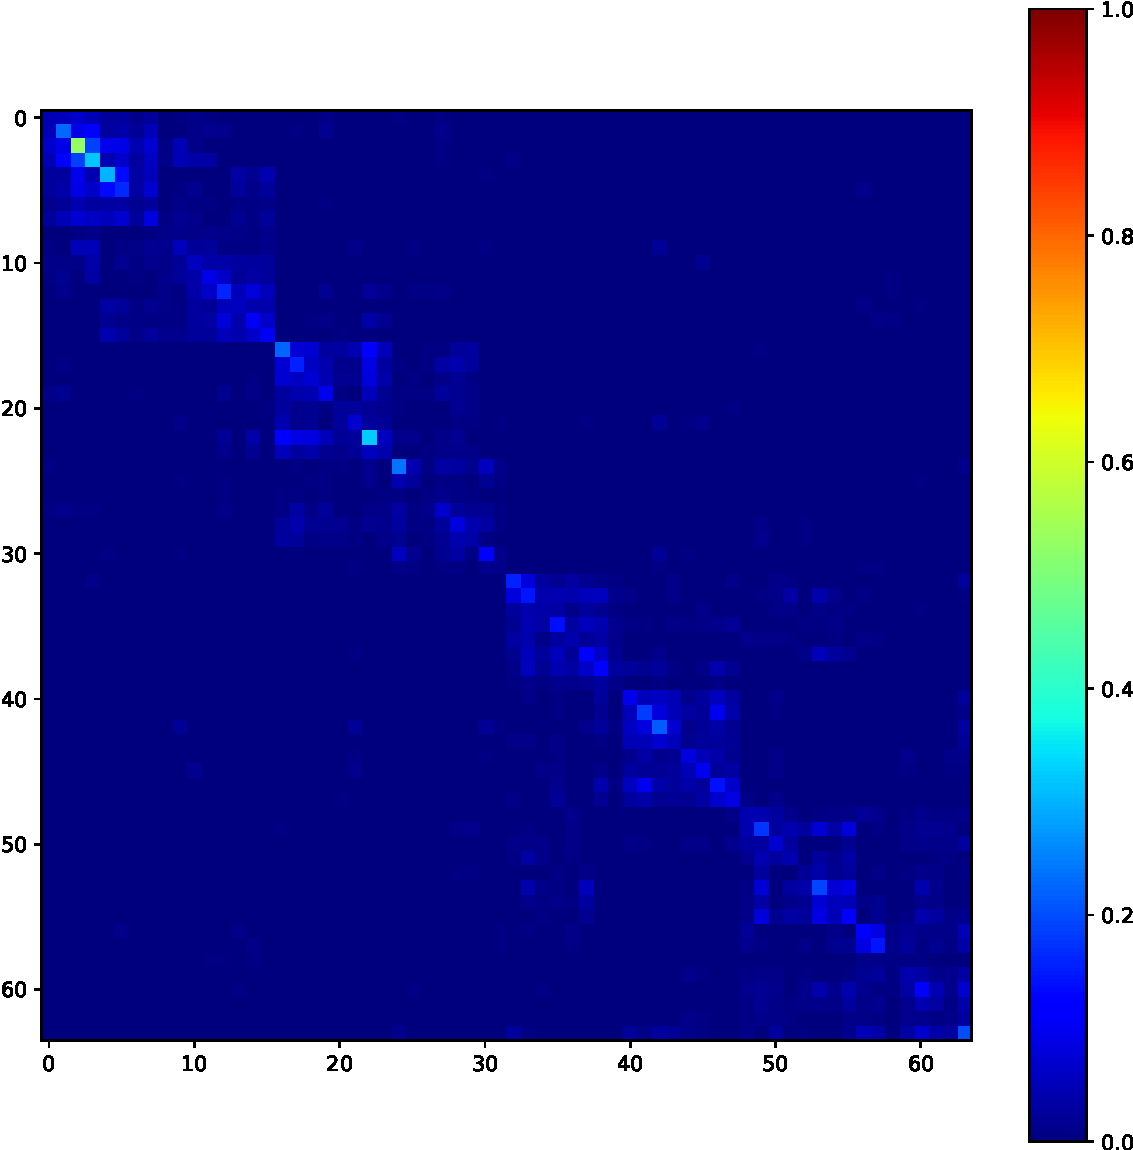
\includegraphics[width=0.5\linewidth]{cov_hme.pdf} \\
		{\footnotesize (b) HME-6}
	\end{tabular}
\end{center}
\caption[Covariance matrix of gating values of generators for ME-64 and HME-6.]{Covariance matrix of gating values of generators for ME-64 and HME-6. We see spectral squares near diagonal for HME-6 model, which indicates generators that are closer by index are used together.}
\vskip\baselineskip
\label{fig:covariances}
\end{figure}

The 5-NN and FID scores for five different data sets are visualized in Figure \ref{fig:box_s1} and \ref{fig:box_s2}. All results are also reported in Tables \ref{tab:res:mnist} to \ref{tab:res:flowers}. The summary of qualitative metrics implies that ME and HME perform around the same. We see that the results for HME generally gets better with the increasing complexity (in terms of number of parameters) as expected. For ME, the results do not get better as in HME. Especially the ME-256 model performs worse than other smaller ME models.

\begin{figure}[htbp]
\begin{center}
	\begin{tabular}{c}
		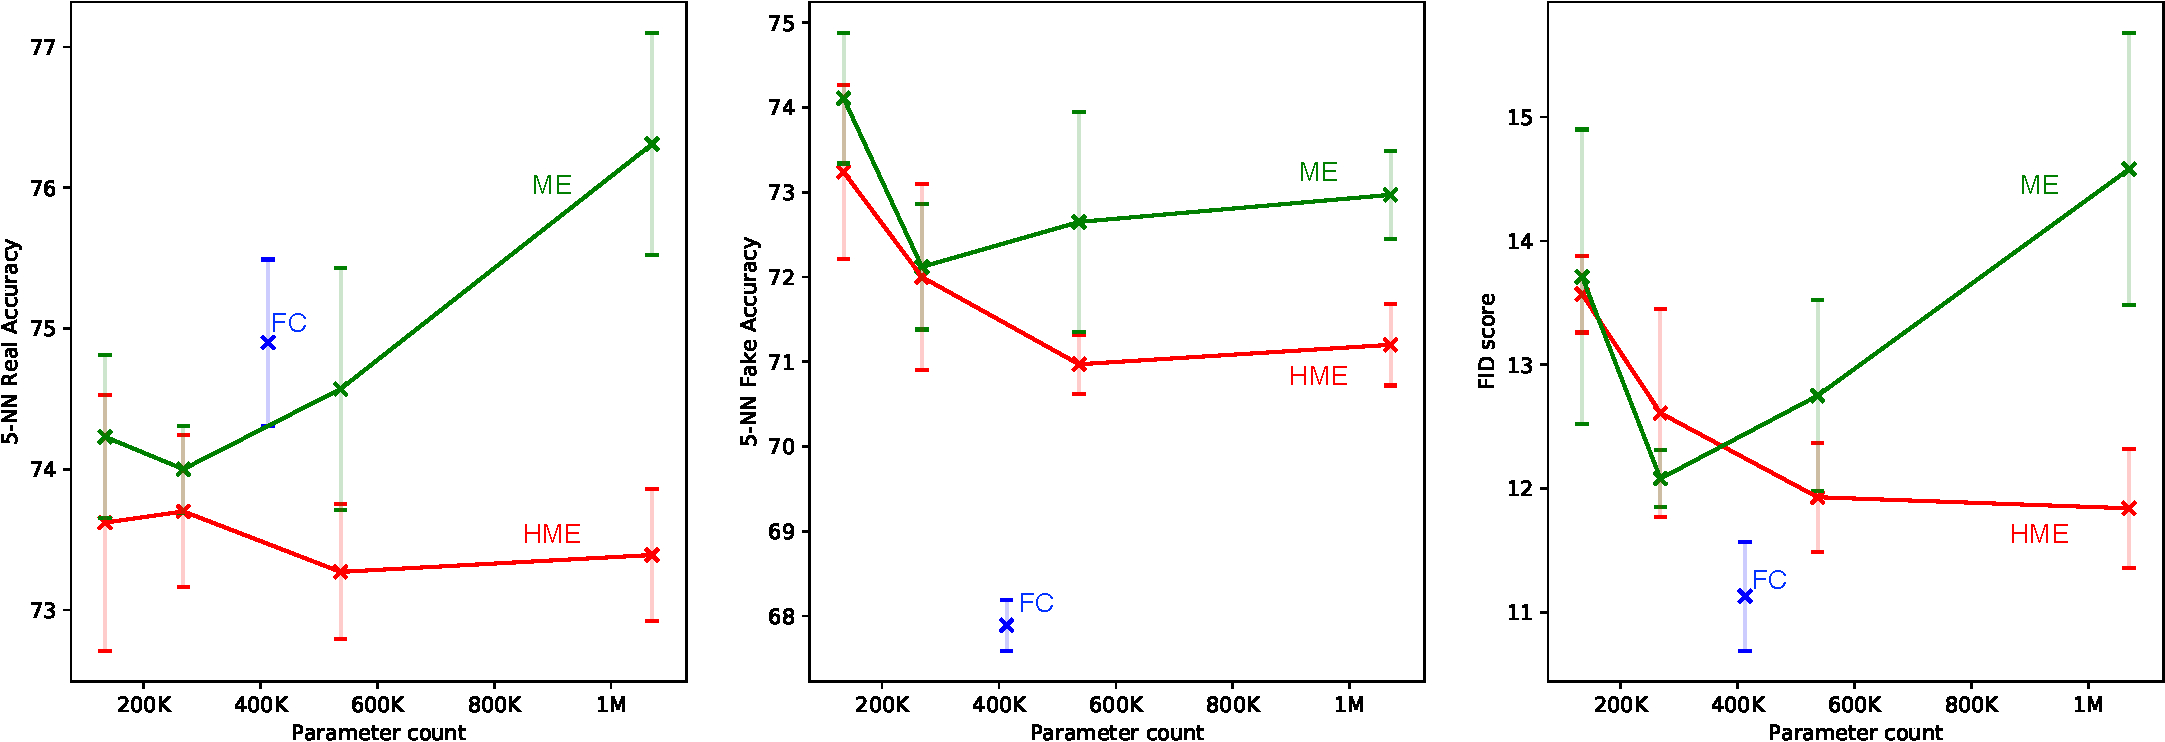
\includegraphics[width=0.95\linewidth]{box_mnist_s.pdf} \\
		{\footnotesize (a) MNIST} \\
		\vspace{0cm} \\
		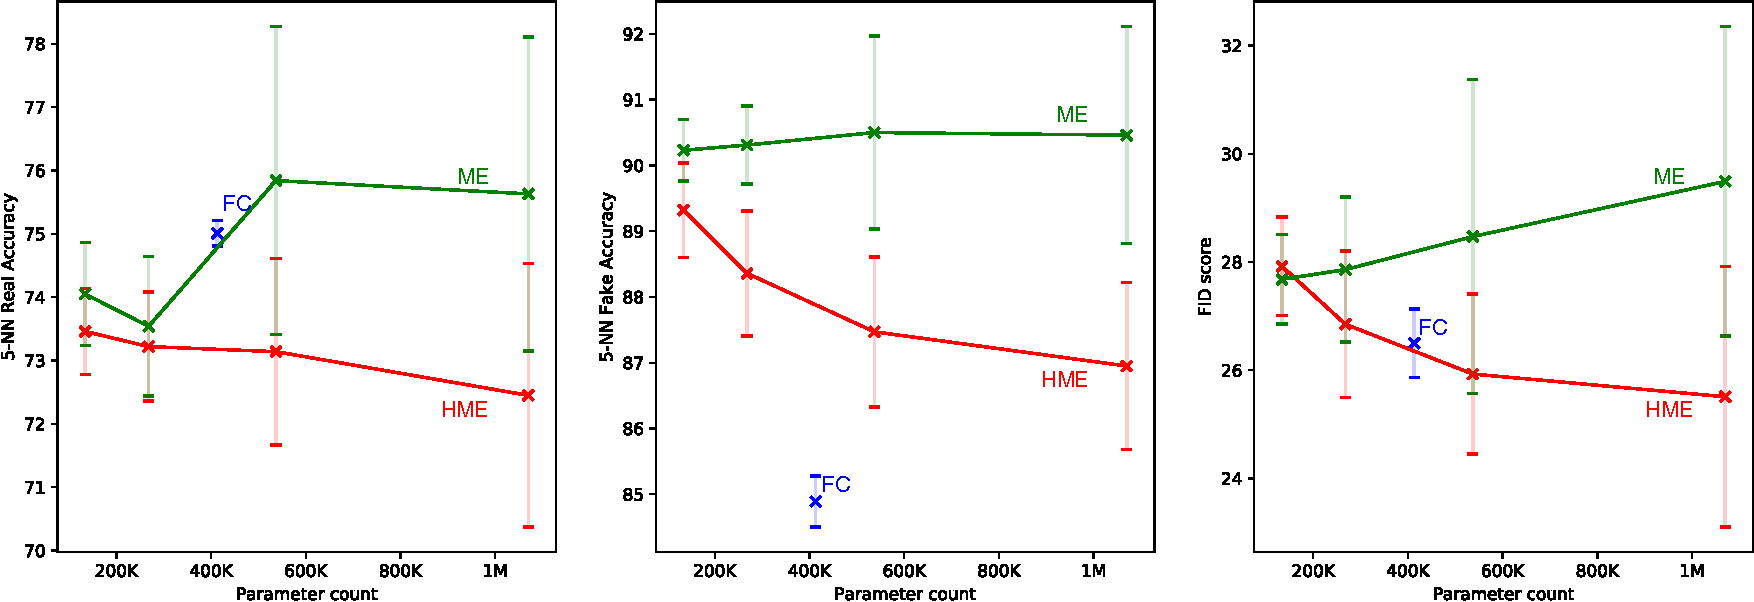
\includegraphics[width=0.95\linewidth]{box_fashion_s.pdf} \\
		{\footnotesize (b) FashionMNIST}
	\end{tabular}
\end{center}
\caption[FID scores and 5-NN accuracies of ME-$k$ and HME-$k$ on MNIST and FashionMNIST]{FID scores and 5-NN accuracies of ME-$k$ and HME-$k$ on MNIST and FashionMNIST data sets. Lower FID and 5-NN scores are better. The parameter count does not include the convolutional part.}
\vskip\baselineskip
\label{fig:box_s1}
\end{figure}

\begin{figure}[htbp]
\begin{center}
	\begin{tabular}{c}
		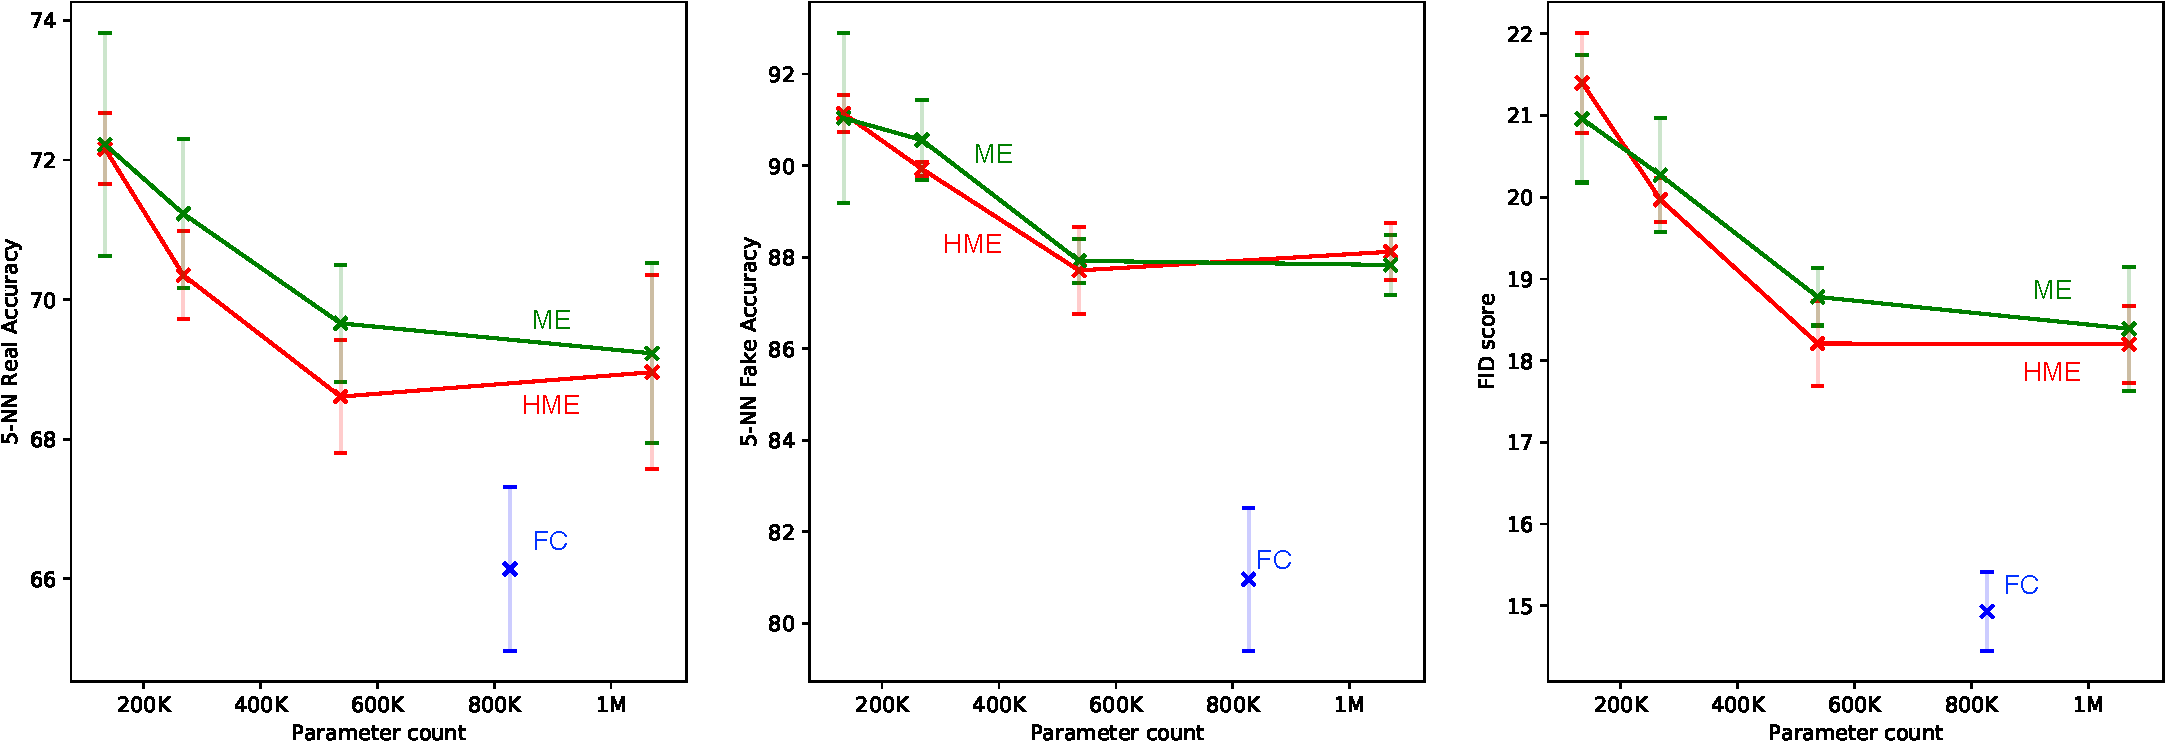
\includegraphics[width=0.95\linewidth]{box_celeb_s.pdf}\\
		{\footnotesize (a) CelebA} \\
		\vspace{0cm} \\
		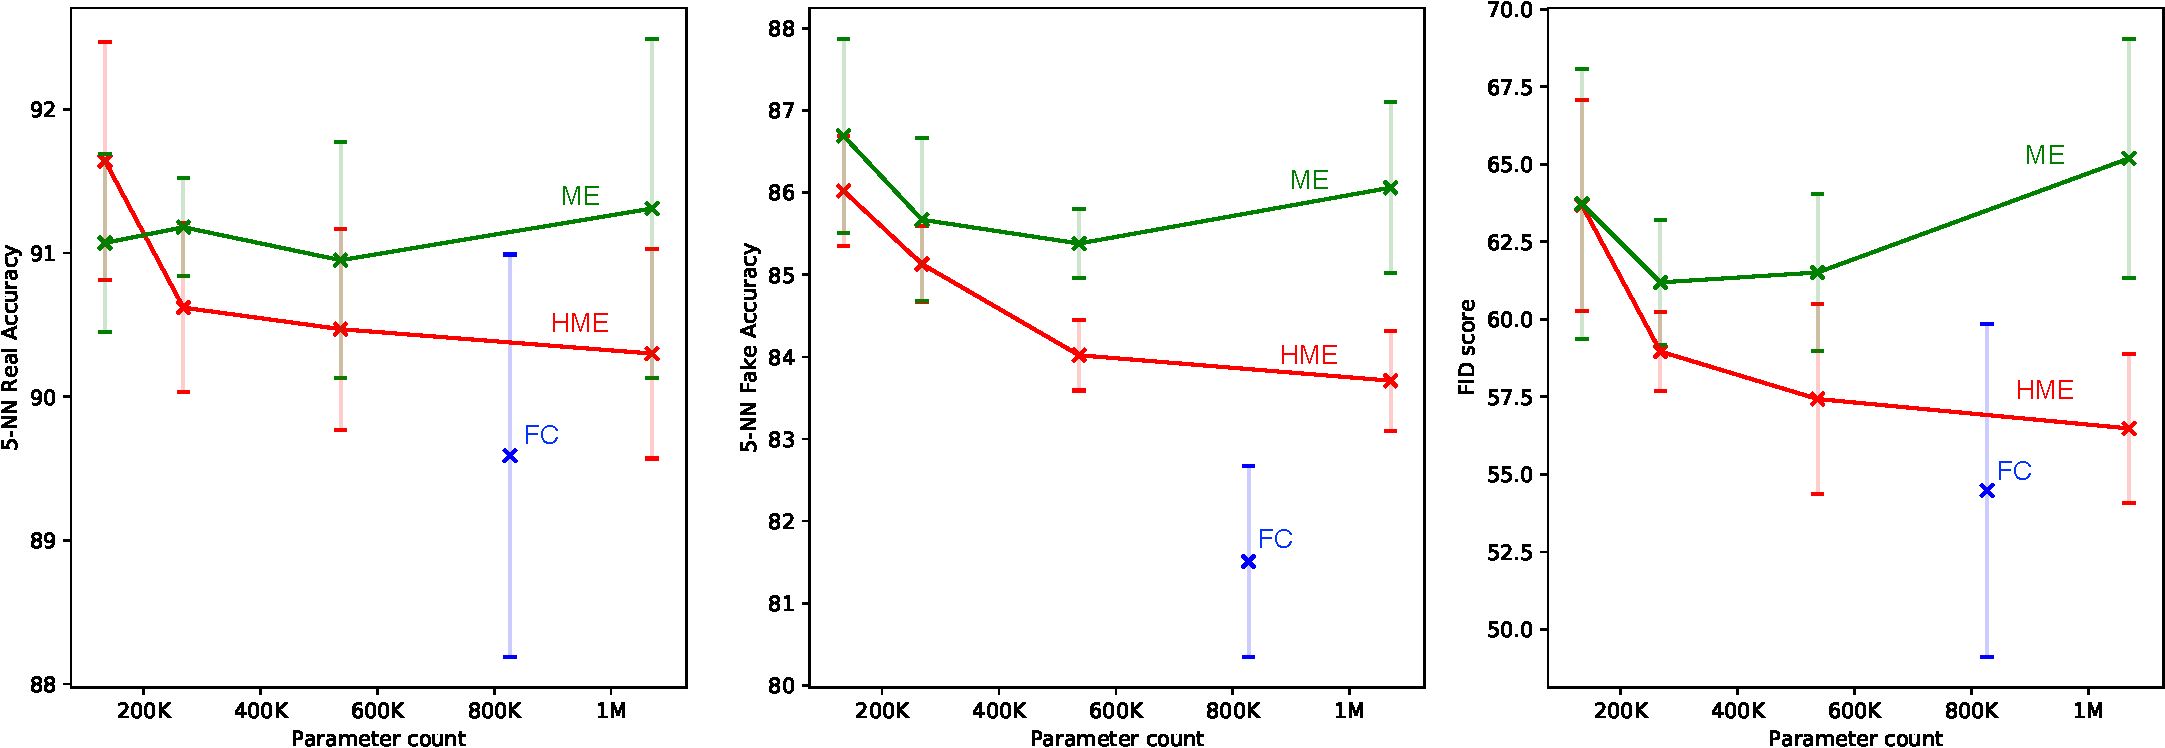
\includegraphics[width=0.95\linewidth]{box_utzap50k_s.pdf}\\
		{\footnotesize (b) UTZap50K} \\
		\vspace{0cm} \\
		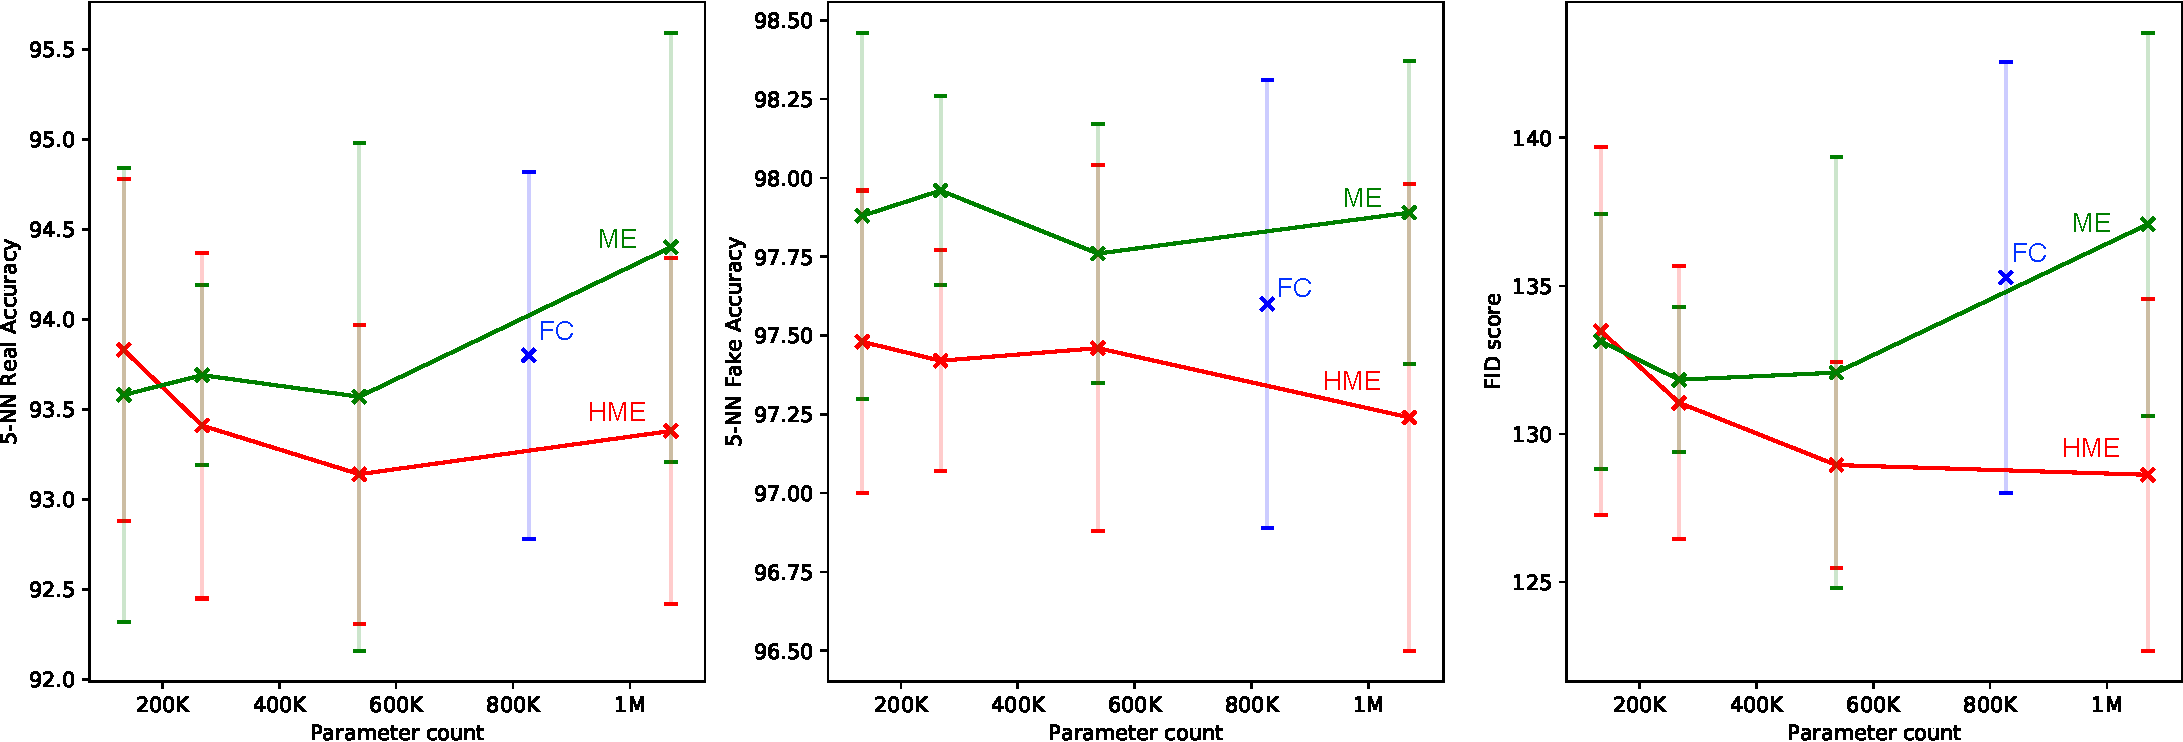
\includegraphics[width=0.95\linewidth]{box_flowers_s.pdf} \\
		{\footnotesize (c) Oxford Flowers}
	\end{tabular}
\end{center}
\caption[FID scores and 5-NN accuracies of ME-$k$ and HME-$k$ on CelebA, UTZap50K, and Oxford Flowers]{FID scores and 5-NN accuracies of ME-$k$ and HME-$k$ on CelebA, UTZap50K, and Oxford Flowers data sets. Lower FID and 5-NN scores are better. The parameter count does not include the convolutional part.}
\vskip\baselineskip
\label{fig:box_s2}
\end{figure}

\begin{table}[thbp]
\vskip\baselineskip
\caption[5-NN accuracies and FID scores of ME and HME models on MNIST data set.]{5-NN accuracies and FID scores of ME and HME models on MNIST.}
\vskip\baselineskip
\begin{center}
\begin{tabular}{|c|c|c|c|c|}
\hline
Model & 5-NN Real & 5-NN Fake & FID & Param. \\
\hline
FC (baseline) & $74.90 \pm 0.59$ & $67.89 \pm 0.30$ & $11.13 \pm 0.44$ & 413K\\
\hline
HME-5 & $73.62 \pm 0.91$ & $73.24 \pm 1.03$ & $13.57 \pm 0.31$ & 134K\\
HME-6 & $73.70 \pm 0.54$ & $72.00 \pm 1.10$ & $12.61 \pm 0.84$ & 268K\\
HME-7 & $73.27 \pm 0.48$ & $70.97 \pm 0.35$ & $11.93 \pm 0.44$ & 537K\\
HME-8 & $73.39 \pm 0.47$ & $71.20 \pm 0.48$ & $11.84 \pm 0.48$ & 1.07M\\
\hline
ME-32 & $74.23 \pm 0.58$ & $74.11 \pm 0.77$ & $13.71 \pm 1.19$ & 134K\\
ME-64 & $74.00 \pm 0.31$ & $72.12 \pm 0.74$ & $12.08 \pm 0.23$ & 268K\\
ME-128 & $74.57 \pm 0.86$ & $72.65 \pm 1.30$ & $12.75 \pm 0.77$ & 537K\\
ME-256 & $76.31 \pm 0.79$ & $72.97 \pm 0.52$ & $14.58 \pm 1.10$ & 1.07M\\
\hline
\end{tabular}
\label{tab:res:mnist}
\end{center}
\end{table}

\begin{table}[thbp]
\vskip\baselineskip
\caption[5-NN accuracies and FID scores of ME and HME models on FashionMNIST data set.]{5-NN accuracies and FID scores of ME and HME models on FashionMNIST.}
\vskip\baselineskip
\begin{center}
\begin{tabular}{|c|c|c|c|c|}
\hline
Model & 5-NN Real & 5-NN Fake & FID & Param. \\
\hline
FC (baseline) & $75.01 \pm 0.20$ & $84.89 \pm 0.39$ & $26.50 \pm 0.63$ & 413K\\
\hline
HME-5 & $73.46 \pm 0.68$ & $89.32 \pm 0.72$ & $27.92 \pm 0.91$ & 134K\\
HME-6 & $73.22 \pm 0.86$ & $88.36 \pm 0.95$ & $26.85 \pm 1.35$ & 268K\\
HME-7 & $73.14 \pm 1.47$ & $87.47 \pm 1.14$ & $25.93 \pm 1.48$ & 537K\\
HME-8 & $72.45 \pm 2.08$ & $86.95 \pm 1.27$ & $25.51 \pm 2.41$ & 1.07M\\
\hline
ME-32 & $74.05 \pm 0.81$ & $90.23 \pm 0.47$ & $27.68 \pm 0.83$ & 134K\\
ME-64 & $73.54 \pm 1.10$ & $90.31 \pm 0.59$ & $27.86 \pm 1.34$ & 268K\\
ME-128 & $75.84 \pm 2.43$ & $90.50 \pm 1.47$ & $28.47 \pm 2.90$ & 537K\\
ME-256 & $75.63 \pm 2.48$ & $90.46 \pm 1.65$ & $29.49 \pm 2.86$ & 1.07M\\
\hline
\end{tabular}
\label{tab:res:fashion}
\end{center}
\end{table}

\begin{table}[thbp]
\vskip\baselineskip
\caption[5-NN accuracies and FID scores of ME and HME models on CelebA data set.]{5-NN accuracies and FID scores of ME and HME models on CelebA.}
\vskip\baselineskip
\begin{center}
\begin{tabular}{|c|c|c|c|c|}
\hline
Model & 5-NN Real & 5-NN Fake & FID & Param. \\
\hline
FC (baseline) & $66.14 \pm 1.17$ & $80.96 \pm 1.56$ & $14.93 \pm 0.48$ & 827K\\
\hline
HME-5 & $72.16 \pm 0.51$ & $91.14 \pm 0.40$ & $21.40 \pm 0.61$ & 265K\\
HME-6 & $70.35 \pm 0.63$ & $89.93 \pm 0.15$ & $19.97 \pm 0.27$ & 530K\\
HME-7 & $68.61 \pm 0.81$ & $87.71 \pm 0.95$ & $18.21 \pm 0.52$ & 1.06M\\
HME-8 & $68.96 \pm 1.39$ & $88.12 \pm 0.62$ & $18.20 \pm 0.47$ & 2.12M\\
\hline
ME-32 & $72.22 \pm 1.60$ & $91.04 \pm 1.86$ & $20.96 \pm 0.78$ & 265K\\
ME-64 & $71.23 \pm 1.07$ & $90.56 \pm 0.87$ & $20.27 \pm 0.70$ & 530K\\
ME-128 & $69.66 \pm 0.84$ & $87.92 \pm 0.48$ & $18.78 \pm 0.35$ & 1.06M\\
ME-256 & $69.23 \pm 1.29$ & $87.83 \pm 0.66$& $18.39 \pm 0.76$ & 2.12M\\
\hline
\end{tabular}
\label{tab:res:celeb}
\end{center}
\end{table}

\begin{table}[thbp]
\vskip\baselineskip
\caption[5-NN accuracies and FID scores of ME and HME models on UTZap 50K data set.]{5-NN accuracies and FID scores of ME and HME models on UTZap50K.}
\vskip\baselineskip
\begin{center}
\begin{tabular}{|c|c|c|c|c|}
\hline
Model & 5-NN Real & 5-NN Fake & FID & Param. \\
\hline
FC (baseline) & $89.59 \pm 1.40$ & $81.51 \pm 1.16$ & $54.48 \pm 5.36$ & 827K\\
\hline
HME-5 & $91.64 \pm 0.83$ & $86.02 \pm 0.67$ & $63.67 \pm 3.40$ & 265K\\
HME-6 & $90.62 \pm 0.59$ & $85.13 \pm 0.46$ & $58.96 \pm 1.28$ & 530K\\
HME-7 & $90.47 \pm 0.70$ & $84.02 \pm 0.43$ & $57.43 \pm 3.06$ & 1.06M\\
HME-8 & $90.30 \pm 0.73$ & $83.71 \pm 0.61$ & $56.48 \pm 2.39$ & 2.12M\\
\hline
ME-32 & $91.07 \pm 0.62$ & $86.69 \pm 1.18$ & $63.72 \pm 4.35$ & 265K\\
ME-64 & $91.18 \pm 0.34$ & $85.67 \pm 0.99$ & $61.19 \pm 2.02$ & 530K\\
ME-128 & $90.95 \pm 0.82$ & $85.38 \pm 0.42$ & $61.51 \pm 2.52$ & 1.06M\\
ME-256 & $91.31 \pm 1.18$ & $86.06 \pm 1.04$ & $65.19 \pm 3.85$ & 2.12M\\
\hline
\end{tabular}
\label{tab:res:utzap50k}
\end{center}
\end{table}

\begin{table}[thbp]
\vskip\baselineskip
\caption[5-NN accuracies and FID scores of ME and HME models on Oxford Flowers data set.]{5-NN accuracies and FID scores of ME and HME models on Oxford Flowers.}
\vskip\baselineskip
\begin{center}
\begin{tabular}{|c|c|c|c|c|}
\hline
Model & 5-NN Real & 5-NN Fake & FID & Param. \\
\hline
FC (baseline) & $93.80 \pm 1.02$ & $97.60 \pm 0.71$ & $135.28 \pm 7.28$ & 827K\\
\hline
HME-5 & $93.83 \pm 0.95$ & $97.48 \pm 0.48$ & $133.47 \pm 6.22$ & 265K\\
HME-6 & $93.41 \pm 0.96$ & $97.42 \pm 0.35$ & $131.05 \pm 4.61$ & 530K\\
HME-7 & $93.14 \pm 0.83$ & $97.46 \pm 0.58$ & $128.95 \pm 3.49$ & 1.06M\\
HME-8 & $93.38 \pm 0.96$ & $97.24 \pm 0.74$ & $128.62 \pm 5.94$ & 2.12M\\
\hline
ME-32 & $93.58 \pm 1.26$ & $97.88 \pm 0.58$ & $133.13 \pm 4.31$ & 265K\\
ME-64 & $93.69 \pm 0.50$ & $97.96 \pm 0.30$ & $131.83 \pm 2.45$ & 530K\\
ME-128 & $93.57 \pm 1.41$ & $97.76 \pm 0.41$ & $132.07 \pm 7.28$ & 1.06M\\
ME-256 & $94.40 \pm 1.19$ & $97.89 \pm 0.48$ & $137.08 \pm 6.46$ & 2.12M\\
\hline
\end{tabular}
\label{tab:res:flowers}
\end{center}
\end{table}

When we make a comparison with the baseline, we see that ME and HME are not as good as FC in terms of FID score or 5-NN accuracy (Figure \ref{fig:box_s1} and \ref{fig:box_s2}). Their performance improves as the structure gets larger; note that trees with depth five and six are smaller than FC. Although 5-NN real accuracies are quite close, there is a gap between 5-NN fake accuracies. High 5-NN fake accuracy implies that fake samples are located near fake samples in $p(x)$. So, the performance drop might be due to decreased sample diversity.

One possible cause for the decreased diversity is to use constant vectors in the leaves. In an FC layer, the random vector $z$ is gone through an affine transformation and a ReLU non-linearity, the \emph{randomness} is propagated linearly. ME and HME, on the other hand, encapsulate the information of $z$ (randomness) in their gating values. Gating values are calculated with a set of sigmoid functions for HME, and with a softmax function for ME. Both the sigmoid function and the softmax function get saturated for values that are too low or too high. Therefore, if gating weights get too high or too low, which also means that it mimics a hard split instead of a soft one, the variety is lost.

To remedy this problem, we use linear functions as in Equation \ref{eq:linear} at leaves of both ME and HME models. We experimented with the number of generators set to 4, 8, 16, and 32. We call these models as ME-L-$k$ and HME-L-$k$ where $k$ is the number of generators for the flat mixture and the depth level for the hierarchical mixture.

\begin{figure}[htbp]
\vskip\baselineskip
\begin{center}
	\begin{tabular}{c}
		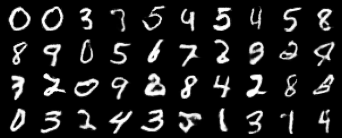
\includegraphics[width=0.75\linewidth]{me_lin_samples_mnist.png}\\
		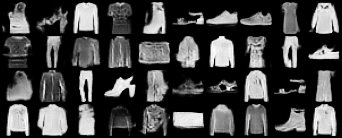
\includegraphics[width=0.75\linewidth]{me_lin_samples_fashion.png}
	\end{tabular}
\end{center}
\caption{Samples generated using ME-L-16 on $32 \times 32$ sized data sets.}
\vskip\baselineskip
\label{fig:samples_lin_me}
\end{figure}

\begin{figure}[htbp]
\begin{center}
	\begin{tabular}{c}
		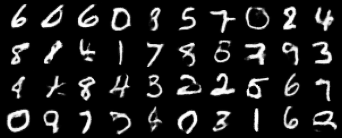
\includegraphics[width=0.75\linewidth]{hme_lin_samples_mnist.png}\\
		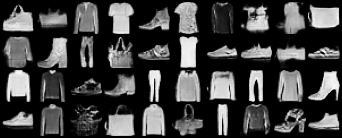
\includegraphics[width=0.75\linewidth]{hme_lin_samples_fashion.png}
	\end{tabular}
\end{center}
\caption{Samples generated using HME-L-4 on $32 \times 32$ sized data sets.}
\vskip\baselineskip
\label{fig:samples_lin_hme}
\end{figure}

\begin{figure}[htbp]
\begin{center}
	\begin{tabular}{c}
		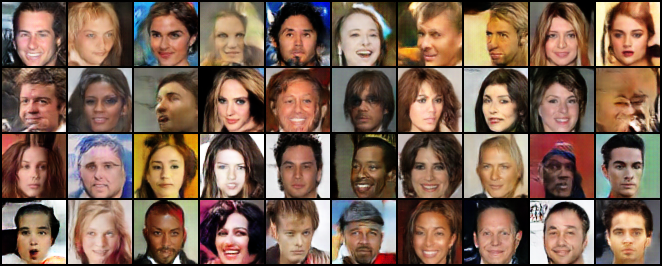
\includegraphics[width=0.9\linewidth]{me_lin_samples_celeb.png}\\
		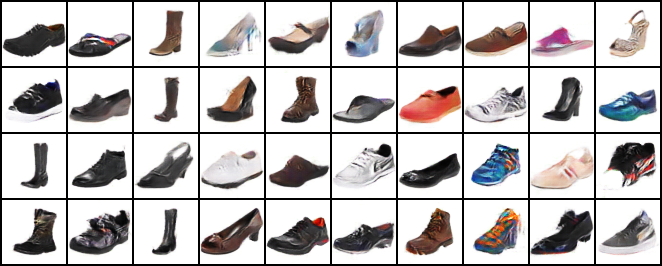
\includegraphics[width=0.9\linewidth]{me_lin_samples_utzap50k.png}\\
		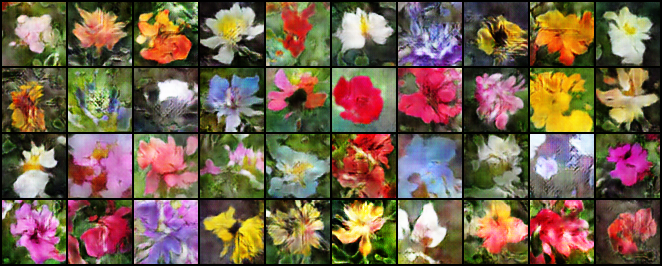
\includegraphics[width=0.9\linewidth]{me_lin_samples_flowers.png}
	\end{tabular}
\end{center}
\caption{Samples generated using ME-L-16 on $64 \times 64$ sized data sets.}
\vskip\baselineskip
\label{fig:samples_lin_me2}
\end{figure}

\begin{figure}[htbp]
\begin{center}
	\begin{tabular}{c}
		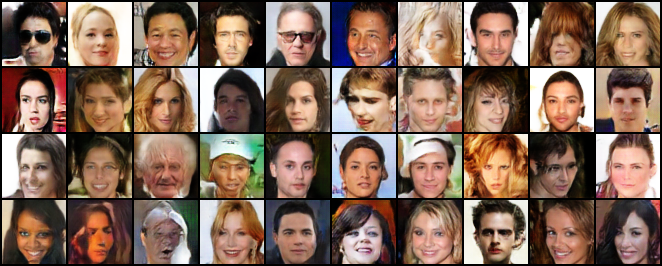
\includegraphics[width=0.9\linewidth]{hme_lin_samples_celeb.png}\\
		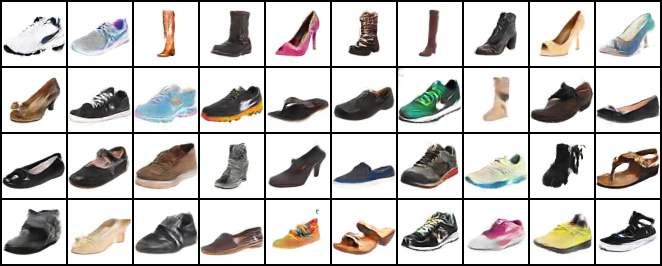
\includegraphics[width=0.9\linewidth]{hme_lin_samples_utzap50k.png}\\
		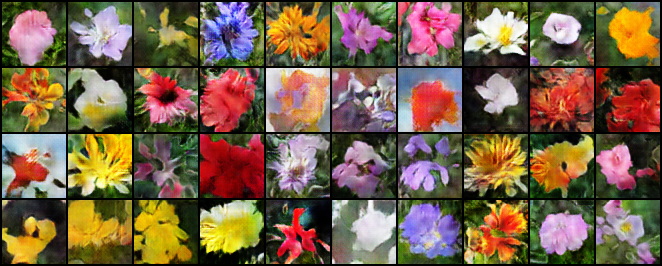
\includegraphics[width=0.9\linewidth]{hme_lin_samples_flowers.png}
	\end{tabular}
\end{center}
\caption{Samples generated using HME-L-4 on $64 \times 64$ sized data sets.}
\vskip\baselineskip
\label{fig:samples_lin_hme2}
\end{figure}

\begin{figure}[htbp]
\begin{center}
	\begin{tabular}{c}
		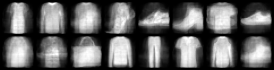
\includegraphics[width=0.9\linewidth]{me_lin_leaves_fashion.png}\\
		{\footnotesize (a) ME-L-16}\\
		\vspace{0cm} \\
		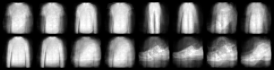
\includegraphics[width=0.9\linewidth]{hme_lin_leaves_fashion.png}\\
		{\footnotesize (b) HME-L-4}
	\end{tabular}
\end{center}
\caption{The average responses of generators at the leaves for ME-L-16 and HME-L-4.}
\vskip\baselineskip
\label{fig:leaves_lin}
\end{figure}

\vskip\baselineskip
The experimental results on five data sets are given in Tables \ref{tab:res:related:mnist} to \ref{tab:res:related:flowers}. First, we see that both ME-L and HME-L models outperform the baseline FC model. Though one can expect these results since the number of parameters increases. Both 5-NN real and 5-NN fake accuracy drops, which says our mixture models fit better to $p(x)$ with more variety. Some samples generated from ME-L-16 and HME-L-4 are visualized in Figures \ref{fig:samples_lin_me} and \ref{fig:samples_lin_hme}.

When we compare ME-L and HME-L models, we see that ME slightly enjoys more from having linear experts. We visualized the average generator responses for FashionMNIST data set in Figure \ref{fig:leaves_lin}. We see that ME-L leaves are now more local and diverse. Figure \ref{fig:covariances_lin}a also confirms this since the diagonal is now more prominent. On the other hand, in Figure \ref{fig:covariances_lin}b HME seems to use its leaves more cooperatively when compared with its constant counterpart. For both formulations, results stagnate at their largest models. We argue that the training time may increase when the number of generators increases since we distribute the error to multiple generators. More generators imply we update generators with smaller gradients.

In Figure \ref{fig:gens} and \ref{fig:gens2}, we show some samples generated from different generators at the leaves of ME-L-16 and HME-L-4. Each generator works in a different input region. To find these input regions, we sample 10,000 input noise vectors and select the top five most likely points. Here, the most likely point for a generator is the point which maximizes the gating value of a generator.

In Figure \ref{fig:gens}, we see that each generator is localized in a different input-output mapping region. When we look at columns from five to eight in Figure \ref{fig:gens}b, they are all digits that contain a vertical stroke. Since HME-L-4 is a tree with a depth of four, generators from five to eight have the same ancestor at the second level of the tree. We see that digits that contain a vertical stroke are split from others at the second level of the tree. These digits are further split into different leaves when we go down at the bottom of the tree. This further confirms our hypothesis that HME hierarchically splits the data generation task. Likewise in Figure \ref{fig:gens2}b, for HME model we see that generators that are neighbors create images that share common features such as background color, hair type, gender. For example, male faces are generally located in the first eight columns which indicates that the tree is softly split by the gender feature at the first level. This is a good split since the split by the gender approximately splits $p(x)$ by half. When we go down in the tree, splits become more detailed. In columns 11 and 12, we see women with different hair colors but with the same orientation and hair type.

\begin{figure}[htbp]
\begin{center}
	\begin{tabular}{c}
		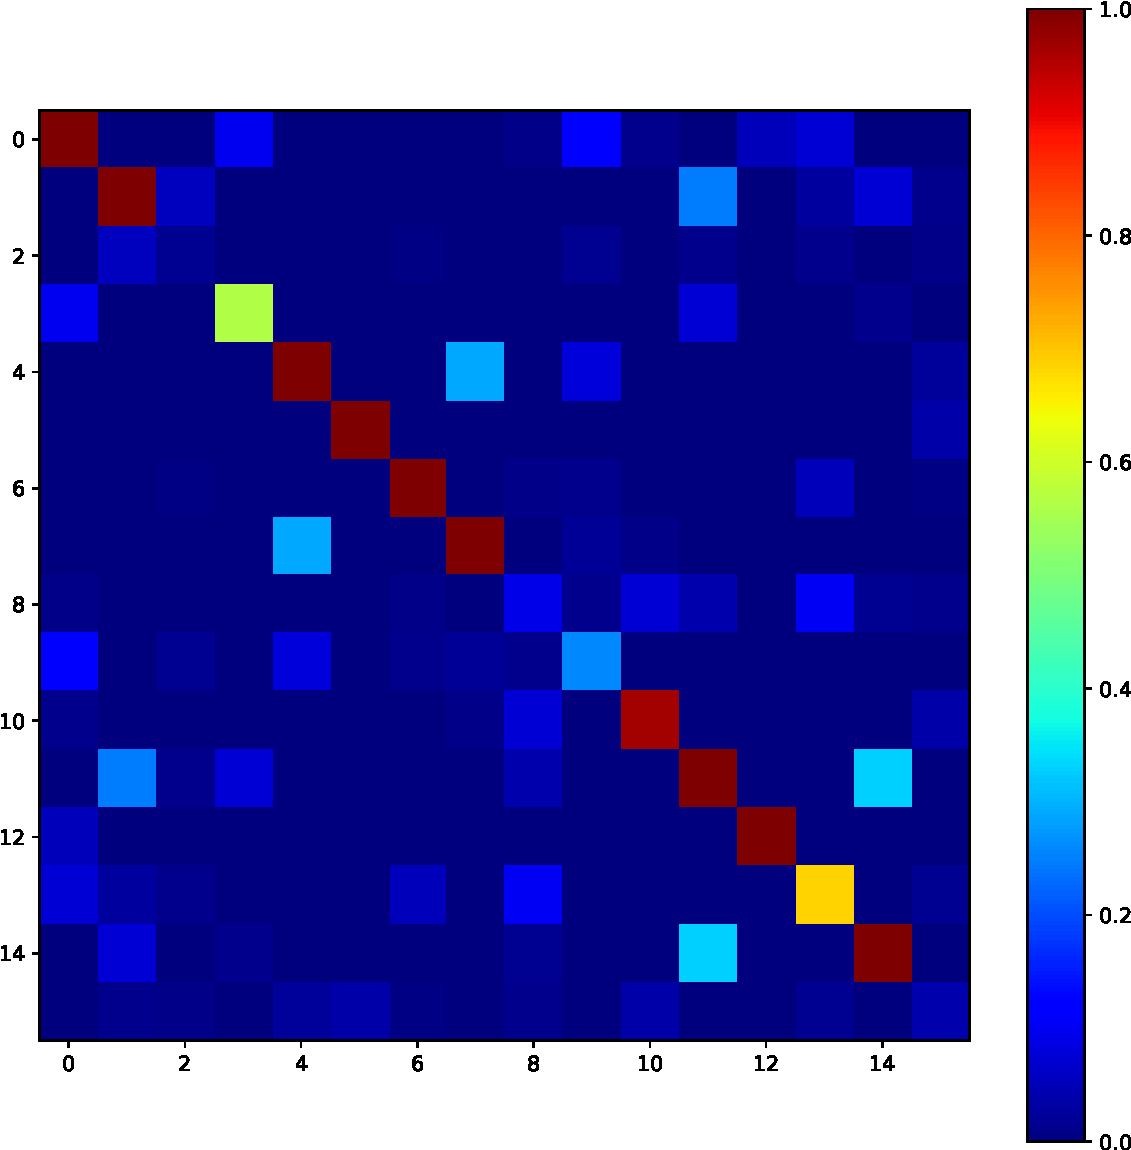
\includegraphics[width=0.5\linewidth]{cov_me_lin.pdf}\\
		{\footnotesize (a) ME-L-16} \\
		\vspace{0cm} \\
		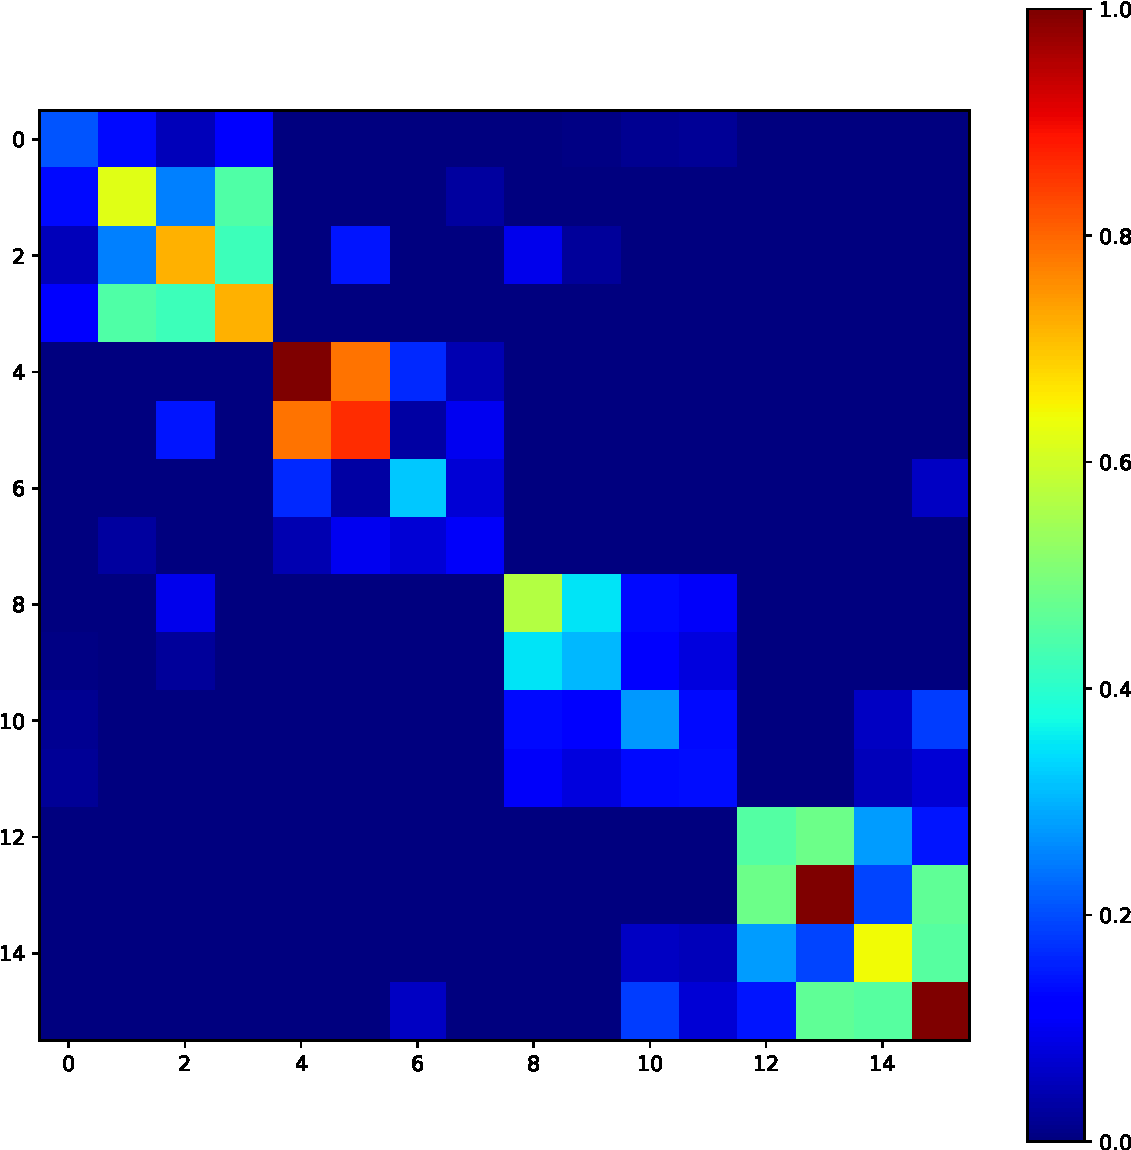
\includegraphics[width=0.5\linewidth]{cov_hme_lin.pdf}\\
		{\footnotesize (b) HME-L-4}
	\end{tabular}
\end{center}
\caption[Covariance matrix of gating values of generators for ME-L-16 and HME-L-4.]{Covariance matrix of gating values of generators for ME-L-16 and HME-L-4. As in Figure \ref{fig:covariances}, we see spectral squares near diagonal for HME-L-4 model.}
\vskip\baselineskip
\label{fig:covariances_lin}
\end{figure}

\begin{figure}[htbp]
\begin{center}
	\begin{tabular}{c}
		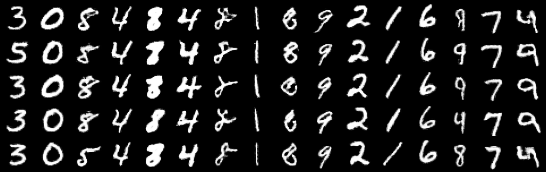
\includegraphics[width=0.95\linewidth]{me_mnist_L4_exps.png} \\
		{\footnotesize (a) ME-L-16} \\
		\vspace{0cm} \\
		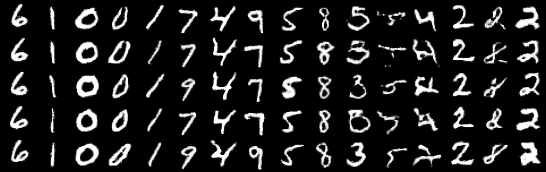
\includegraphics[width=0.95\linewidth]{hme_mnist_L4_exps.png} \\
		{\footnotesize (b) HME-L-4}
	\end{tabular}
\end{center}
\caption[Some samples generated from generators at the leaves of ME-L-16 and HME-L-4 for MNIST data set.]{Some samples generated from generators at the leaves of ME-L-16 and HME-L-4 for MNIST data set. Samples in the $i$th column are generated from $i$th generator.}
\vskip\baselineskip
\label{fig:gens}
\end{figure}

\begin{figure}[htbp]
\begin{center}
	\begin{tabular}{c}
		\includegraphics[width=0.95\linewidth]{me_celeb_L4_exps.png} \\
		{\footnotesize (a) ME-L-16} \\
		\vspace{0cm} \\
		\includegraphics[width=0.95\linewidth]{hme_celeb_L4_exps.png}\\
		{\footnotesize (b) HME-L-4}
	\end{tabular}
\end{center}
\caption[Some samples generated from generators at the leaves of ME-L-16 and HME-L-4 for CelebA data set.]{Some samples generated from generators at the leaves of ME-L-16 and HME-L-4 for CelebA data set. Samples in the $i$th column are generated from $i$th generator.}
\vskip\baselineskip
\label{fig:gens2}
\end{figure}

\section{Comparison with Related Works}
\label{sec:related_results}
In this section, we compare our models with related works that we mentioned in Chapter \ref{chapter:multiple_gan}. We test each method for different number of generators. MADGAN-$k$, MGAN-$k$, MEGAN-$k$ and ME-GAN-$k$ denote models with $k$ generators. We also report the parameter count of each model; these do not include the convolution parameters shared across all models. Our experiment results on five different data sets are summarized in Figures \ref{fig:box1} and \ref{fig:box2}. We also report the results in Tables \ref{tab:res:related:mnist} to \ref{tab:res:related:flowers}.

%%
\begin{table}[thbp]
\vskip\baselineskip
\caption[5-NN accuracies and FID scores on MNIST data set.]{5-NN accuracies and FID scores on MNIST.}
\vskip\baselineskip
\begin{center}
\begin{tabular}{|c|c|c|c|c|}
\hline
Model & 5-NN Real & 5-NN Fake & FID & Param. \\
\hline
FC (baseline) & $74.90 \pm 0.59$ & $67.89 \pm 0.30$ & $11.13 \pm 0.44$ & 413K\\
\hline
HME-L-2 & $74.03 \pm 0.81$ & $66.73 \pm 0.61$ & $10.27 \pm 0.41$ & 1.65M\\
HME-L-3 & $73.48 \pm 0.53$ & $66.41 \pm 0.74$ & $9.86 \pm 0.24$ & 3.31M\\
HME-L-4 & $72.10 \pm 0.74$ & $66.21 \pm 0.82$ & $9.15 \pm 0.45$ & 6.62M\\
HME-L-5 & $72.14 \pm 0.54$ & $65.63 \pm 0.25$ & $9.07 \pm 0.44$ & 13.24M\\
\hline
ME-L-4 & $72.91 \pm 0.93$ & $66.29 \pm 0.97$ & $9.74 \pm 0.64$ & 1.65M\\
ME-L-8 & $71.46 \pm 1.02$ & $66.25 \pm 0.72$ & $8.95 \pm 0.28$ & 3.31M\\
ME-L-16 & $70.91 \pm 0.83$ & $65.38 \pm 0.70$ & $8.56 \pm 0.53$ & 6.62M\\
ME-L-32 & $71.68 \pm 0.60$ & $65.86 \pm 0.84$ & $8.90 \pm 0.56$ & 13.24M\\
\hline
MADGAN-4 & $75.30 \pm 2.51$ & $73.59 \pm 1.50$ & $10.87 \pm 1.29$ & 1.68M\\
MADGAN-8 & $74.25 \pm 3.50$ & $74.28 \pm 2.46$ & $10.59 \pm 1.26$ & 3.37M\\
MADGAN-16 & $70.40 \pm 2.01$ & $73.02 \pm 1.07$ & $8.64 \pm 0.55$ & 6.75M\\
MADGAN-32 & $67.96 \pm 2.37$ & $75.00 \pm 2.66$ & $7.97 \pm 0.34$ & 13.50M\\
\hline
MGAN-4 & $82.26 \pm 2.00$ & $80.95 \pm 2.59$ & $14.87 \pm 1.09$ & 1.68M\\
MGAN-8 & $82.09 \pm 3.01$ & $82.88 \pm 4.44$ & $14.81 \pm 1.84$ & 3.37M\\
MGAN-16 & $83.32 \pm 4.32$ & $83.01 \pm 4.05$ & $17.16 \pm 5.82$ & 6.75M\\
MGAN-32 & $87.60 \pm 2.32$ & $90.82 \pm 2.73$ & $24.60 \pm 3.82$ & 13.50M\\
\hline
MEGAN-4 & $80.99 \pm 3.41$ & $85.34 \pm 2.26$ & $14.16 \pm 1.91$ & 2.09M\\
MEGAN-8 & $77.65 \pm 2.62$ & $85.38 \pm 1.80$ & $12.11 \pm 1.92$ & 3.79M\\
MEGAN-16 & $73.11 \pm 3.59$ & $82.88 \pm 3.98$ & $9.85 \pm 1.90$ & 7.18M\\
MEGAN-32 & $73.47 \pm 2.61$ & $86.23 \pm 3.17^+$ & $10.53 \pm 1.69$ & 14.01M\\
\hline
\end{tabular}
\label{tab:res:related:mnist}
\end{center}
\end{table}
%%
\begin{table}[thbp]
\vskip\baselineskip
\caption[5-NN accuracies and FID scores on FashionMNIST data set.]{5-NN accuracies and FID scores on FashionMNIST.}
\vskip\baselineskip
\begin{center}
\begin{tabular}{|c|c|c|c|c|}
\hline
Model & 5-NN Real & 5-NN Fake & FID & Param. \\
\hline
FC (baseline) & $75.01 \pm 0.20$ & $84.89 \pm 0.39$ & $26.50 \pm 0.63$ & 413K\\
\hline
HME-L-2 & $72.18 \pm 0.38$ & $79.96 \pm 0.35$ & $20.88 \pm 0.17$ & 1.65M\\
HME-L-3 & $71.15 \pm 0.88$ & $79.14 \pm 0.73$ & $19.64 \pm 0.89$ & 3.31M\\
HME-L-4 & $70.08 \pm 0.84$ & $78.67 \pm 0.78$ & $18.79 \pm 0.77$ & 6.62M\\
HME-L-5 & $69.99 \pm 0.70$ & $78.10 \pm 0.60$ & $18.24 \pm 0.91$ & 13.24M\\
\hline
ME-L-4 & $72.28 \pm 0.60$ & $79.81 \pm 0.93$ & $20.90 \pm 0.87$ & 1.65M\\
ME-L-8 & $70.90 \pm 0.96$ & $78.64 \pm 0.51$ & $19.37 \pm 0.90$ & 3.31M\\
ME-L-16 & $69.45 \pm 0.71$ & $78.09 \pm 0.73$ & $18.09 \pm 0.89$ & 6.62M\\
ME-L-32 & $70.18 \pm 0.94$ & $79.10 \pm 0.86$ & $19.28 \pm 0.67$ & 13.24M\\
\hline
MADGAN-4 & $86.98 \pm 0.91$ & $93.72 \pm 1.07$ & $39.72 \pm 2.95$ & 1.68M\\
MADGAN-8 & $85.22 \pm 1.82$ & $93.64 \pm 1.13$ & $36.47 \pm 2.40$ & 3.37M\\
MADGAN-16 & $81.95 \pm 1.95$ & $91.80 \pm 1.27$ & $31.54 \pm 3.48$ & 6.75M\\
MADGAN-32 & $82.16 \pm 1.28$ & $93.18 \pm 1.18$ & $33.93 \pm 2.75$ & 13.50M\\
\hline
MGAN-4 & $88.14 \pm 1.55$ & $94.50 \pm 0.70$ & $42.82 \pm 3.50$ & 1.68M\\
MGAN-8 & $87.87 \pm 1.24$ & $94.97 \pm 0.87$ & $41.68 \pm 3.34$ & 3.37M\\
MGAN-16 & $87.10 \pm 1.08$ & $95.32 \pm 0.39$ & $42.72 \pm 1.66$ & 6.75M\\
MGAN-32 & $89.64 \pm 0.69$ & $97.22 \pm 0.85$ & $51.19 \pm 3.91$ & 13.50M\\
\hline
MEGAN-4 & $84.59 \pm 0.47$ & $92.49 \pm 0.30$ & $36.32 \pm 2.10$ & 2.09M\\
MEGAN-8 & $82.04 \pm 0.40$ & $92.57 \pm 0.60$ & $31.75 \pm 0.61$ & 3.79M\\
MEGAN-16 & $80.44 \pm 1.98$ & $92.58 \pm 1.10$ & $29.52 \pm 3.19$ & 7.18M\\
MEGAN-32 & $79.44 \pm 3.32$ & $93.08 \pm 1.09$ & $28.53 \pm 3.31$ & 14.01M\\
\hline
\end{tabular}
\label{tab:res:related:fashion}
\end{center}
\end{table}
%%
\begin{table}[thbp]
\vskip\baselineskip
\caption[5-NN accuracies and FID scores on CelebA data set.]{5-NN accuracies and FID scores on CelebA.}
\vskip\baselineskip
\begin{center}
\begin{tabular}{|c|c|c|c|c|}
\hline
Model & 5-NN Real & 5-NN Fake & FID & Param. \\
\hline
FC (baseline) & $66.14 \pm 1.17$ & $80.96 \pm 1.56$ & $14.93 \pm 0.48$ & 827K\\
\hline
HME-L-2 & $62.96 \pm 0.81$ & $77.91 \pm 0.83$ & $12.41 \pm 0.40$ & 3.30M\\
HME-L-3 & $63.15 \pm 1.42$ & $77.68 \pm 1.91$ & $12.48 \pm 0.65$ & 6.61M\\
HME-L-4 & $62.07 \pm 0.88$ & $77.18 \pm 0.82$ & $12.23 \pm 0.56$ & 13.23M\\
HME-L-5 & $62.02 \pm 1.02$ & $77.02 \pm 0.98$ & $12.09 \pm 0.56$ & 26.47M\\
\hline
ME-L-4 & $62.56 \pm 0.88$ & $77.87 \pm 1.33$ & $12.30 \pm 0.56$ & 3.30M\\
ME-L-8 & $61.44 \pm 1.27$ & $77.36 \pm 0.50$ & $11.99 \pm 0.27$ & 6.61M\\
ME-L-16 & $62.63 \pm 0.67$ & $78.11 \pm 0.96$ & $12.41 \pm 0.45$ & 13.23M\\
ME-L-32 & $63.01 \pm 1.08$ & $77.74 \pm 1.31$ & $12.64 \pm 0.63$ & 26.47M\\
\hline
MADGAN-4 & $77.87 \pm 2.38$ & $94.91 \pm 2.15$ & $26.91 \pm 4.03$ & 3.37M\\
MADGAN-8 & $74.21 \pm 2.68$ & $92.33 \pm 1.78$ & $23.12 \pm 2.80$ & 6.75M\\
MADGAN-16 & $71.22 \pm 1.55$ & $90.55 \pm 1.18$ & $22.28 \pm 0.55$ & 13.50M\\
MADGAN-32 & $69.46 \pm 2.09$ & $87.94 \pm 0.86$ & $20.16 \pm 1.42$ & 27.00M\\
\hline
MGAN-4 & $76.50 \pm 1.28$ & $96.72 \pm 0.76$ & $33.56 \pm 3.78$ & 3.37M\\
MGAN-8 & $76.42 \pm 1.87$ & $96.05 \pm 2.13$ & $31.46 \pm 3.55$ & 6.75M\\
MGAN-16 & $75.37 \pm 3.79$ & $96.94 \pm 1.34$ & $34.62 \pm 6.14$ & 13.50M\\
MGAN-32 & $94.55 \pm 1.33$ & $99.97 \pm 0.02$ & $73.38 \pm 8.15$ & 27.00M\\
\hline
MEGAN-4 & $61.20 \pm 2.04$ & $87.20 \pm 1.11$ & $13.69 \pm 0.67$ & 4.19M\\
MEGAN-8 & $60.83 \pm 2.06$ & $88.59 \pm 0.42$ & $14.46 \pm 0.73$ & 7.57M\\
MEGAN-16 & $61.67 \pm 1.96$ & $90.30 \pm 0.48$ & $15.36 \pm 0.58$ & 14.34M\\
MEGAN-32 & $65.72 \pm 2.25$ & $95.60 \pm 1.20$ & $19.41 \pm 1.24$ & 27.92M\\
\hline
\end{tabular}
\label{tab:res:related:celeb}
\end{center}
\end{table} 
%%
\begin{table}[thbp]
\vskip\baselineskip
\caption[5-NN accuracies and FID scores on UTZap50K data set.]{5-NN accuracies and FID scores on UTZap50K.}
\vskip\baselineskip
\begin{center}
\begin{tabular}{|c|c|c|c|c|}
\hline
Model & 5-NN Real & 5-NN Fake & FID & Param. \\
\hline
FC (baseline) & $89.59 \pm 1.40$ & $81.51 \pm 1.16$ & $54.48 \pm 5.36$ & 827K\\
\hline
HME-L-2 & $87.26 \pm 0.80$ & $77.46 \pm 1.09$ & $42.35 \pm 3.27$ & 3.30M\\
HME-L-3 & $87.39 \pm 0.96$ & $78.21 \pm 0.32$ & $42.99 \pm 2.08$ & 6.61M\\
HME-L-4 & $87.61 \pm 1.21$ & $78.10 \pm 0.43$ & $44.88 \pm 3.48$ & 13.23M\\
HME-L-5 & $87.77 \pm 1.17$ & $78.42 \pm 1.36$ & $45.54 \pm 3.46$ & 26.47M\\
\hline
ME-L-4 & $87.30 \pm 1.27$ & $77.82 \pm 1.40$ & $43.05 \pm 3.83$ & 3.30M\\
ME-L-8 & $86.83 \pm 1.12$ & $77.25 \pm 1.53$ & $41.95 \pm 2.82$ & 6.61M\\
ME-L-16 & $86.97 \pm 0.54$ & $77.50 \pm 1.13$ & $41.45 \pm 1.99$ & 13.23M\\
ME-L-32 & $87.68 \pm 0.76$ & $77.96 \pm 0.68$ & $44.80 \pm 2.39$ & 26.47M\\
\hline
MADGAN-4 & $98.78 \pm 0.28$ & $96.48 \pm 0.81$ & $123.40 \pm 10.00$ & 3.37M\\
MADGAN-8 & $98.69 \pm 0.39$ & $96.36 \pm 1.84$ & $120.72 \pm 15.21$ & 6.75M\\
MADGAN-16 & $98.33 \pm 0.39$ & $95.33 \pm 0.98$ & $113.06 \pm 9.51$ & 13.50M\\
MADGAN-32 & $97.78 \pm 1.00$ & $95.13 \pm 2.80$ & $112.34 \pm 24.69$ & 27.00M\\
\hline
MGAN-4 & $98.97 \pm 0.49$ & $97.24 \pm 1.54$ & $136.08 \pm 17.81$ & 3.37M\\
MGAN-8 & $99.32 \pm 0.26$ & $98.66 \pm 0.81$ & $153.28 \pm 15.75$ & 6.75M\\
MGAN-16 & $99.59 \pm 0.13$ & $99.38 \pm 0.54$ & $167.76 \pm 17.43$ & 13.50M\\
MGAN-32 & $99.72 \pm 0.10$ & $99.83 \pm 0.10$ & $184.21 \pm 10.32$ & 27.00M\\
\hline
MEGAN-4 & $92.67 \pm 0.85$ & $87.16 \pm 1.50$ & $58.49 \pm 5.52$ & 4.19M\\
MEGAN-8 & $92.52 \pm 1.04$ & $88.90 \pm 1.63$ & $59.14 \pm 4.22$ & 7.57M\\
MEGAN-16 & $92.10 \pm 1.09$ & $90.16 \pm 1.82$ & $59.00 \pm 5.40$ & 14.34M\\
MEGAN-32 & $95.20 \pm 1.03$ & $96.33 \pm 0.39$ & $86.43 \pm 11.55$ & 27.92M\\
\hline
\end{tabular}
\label{tab:res:related:utzap50k}
\end{center}
\end{table}
%%
\begin{table}[thbp]
\vskip\baselineskip
\caption[5-NN accuracies and FID scores on Oxford Flowers data set.]{5-NN accuracies and FID scores on Oxford Flowers.}
\vskip\baselineskip
\begin{center}
\begin{tabular}{|c|c|c|c|c|}
\hline
Model & 5-NN Real & 5-NN Fake & FID & Param. \\
\hline
FC (baseline) & $93.80 \pm 1.02$ & $97.60 \pm 0.71$ & $135.28 \pm 7.28$ & 827K\\
\hline
HME-L-2 & $88.96 \pm 0.93$ & $96.58 \pm 0.58$ & $111.06 \pm 4.84$ & 3.30M\\
HME-L-3 & $89.30 \pm 1.49$ & $96.43 \pm 0.65$ & $111.85 \pm 3.65$ & 6.61M\\
HME-L-4 & $88.89 \pm 1.51$ & $96.61 \pm 0.41$ & $112.78 \pm 3.13$ & 13.23M\\
HME-L-5 & $90.15 \pm 1.60$ & $96.55 \pm 0.76$ & $114.79 \pm 4.20$ & 26.47M\\
\hline
ME-L-4 & $89.25 \pm 2.64$ & $96.84 \pm 0.85$ & $112.05 \pm 6.88$ & 3.30M\\
ME-L-8 & $88.59 \pm 1.43$ & $96.79 \pm 0.69$ & $113.37 \pm 3.92$ & 6.61M\\
ME-L-16 & $89.33 \pm 1.39$ & $96.93 \pm 0.36$ & $115.45 \pm 3.02$ & 13.23M\\
ME-L-32 & $90.12 \pm 1.17$ & $97.11 \pm 0.80$ & $118.00 \pm 4.52$ & 26.47M\\
\hline
MADGAN-4 & $93.70 \pm 1.52$ & $98.47 \pm 0.66$ & $150.46 \pm 9.03$ & 3.37M\\
MADGAN-8 & $91.50 \pm 1.50$ & $98.29 \pm 0.32$ & $137.43 \pm 6.85$ & 6.75M\\
MADGAN-16 & $92.36 \pm 1.09$ & $98.40 \pm 0.20$ & $141.20 \pm 6.56$ & 13.50M\\
MADGAN-32 & $92.92 \pm 0.93$ & $98.71 \pm 0.23$ & $142.47 \pm 2.85$ & 27.00M\\
\hline
MGAN-4 & $94.76 \pm 0.87$ & $99.03 \pm 0.25$ & $154.95 \pm 8.52$ & 3.37M\\
MGAN-8 & $94.54 \pm 0.98$ & $99.21 \pm 0.16$ & $152.33 \pm 5.20$ & 6.75M\\
MGAN-16 & $94.10 \pm 2.03$ & $99.26 \pm 0.22$ & $152.38 \pm 10.83$ & 13.50M\\
MGAN-32 & $95.08 \pm 0.50$ & $99.34 \pm 0.12$ & $157.90 \pm 8.02$ & 27.00M\\
\hline
MEGAN-4 & $87.04 \pm 1.70$ & $96.29 \pm 0.50$ & $104.75 \pm 3.00$ & 4.19M\\
MEGAN-8 & $85.83 \pm 1.34$ & $96.45 \pm 0.70$ & $104.04 \pm 2.75$ & 7.57M\\
MEGAN-16 & $85.67 \pm 1.50$ & $96.71 \pm 0.68$ & $106.73 \pm 4.21$ & 14.34M\\
MEGAN-32 & $85.80 \pm 1.27$ & $97.23 \pm 0.26$ & $107.37 \pm 3.72$ & 27.92M\\
\hline
\end{tabular}
\label{tab:res:related:flowers}
\end{center}
\end{table}
%%%%%%%%%%%%%
\begin{figure}[htbp]
\begin{center}
	\begin{tabular}{c}
		\includegraphics[width=0.95\linewidth]{box_mnist.pdf}\\
		{\footnotesize (a) MNIST} \\
		\vspace{0cm} \\
		\includegraphics[width=0.95\linewidth]{box_fashion.pdf} \\
		{\footnotesize (b) FashionMNIST}
	\end{tabular}
\end{center}
\caption[FID scores and 5-NN accuracies on MNIST and FashionMNIST.]{FID scores and 5-NN accuracies on MNIST and FashionMNIST data sets. The parameter count does not include the convolutional part.}
\vskip\baselineskip
\label{fig:box1}
\end{figure}

\begin{figure}[htbp]
\begin{center}
	\begin{tabular}{c}
		\includegraphics[width=0.95\linewidth]{box_celeb.pdf} \\ 
		{\footnotesize (a) CelebA}\\
		\vspace{0cm} \\
		\includegraphics[width=0.95\linewidth]{box_utzap50k.pdf} \\
		{\footnotesize (b) UTZap50K} \\
		\vspace{0cm} \\
		\includegraphics[width=0.95\linewidth]{box_flowers.pdf} \\
		{\footnotesize (c) Oxford Flowers}
	\end{tabular}
\end{center}
\caption[FID scores and 5-NN accuracies on CelebA, UTZap50K, and Oxford Flowers]{FID scores and 5-NN accuracies on CelebA, UTZap50K, and Oxford Flowers data sets. The parameter count does not include the convolutional part.}
\vskip\baselineskip
\label{fig:box2}
\end{figure}

From the results, we see that MADGAN and MGAN perform worse than the baseline in terms of FID score. Only on the MNIST data set, MADGAN performs better than the baseline. This might suggest that forcing discriminator to classify generators may not always work, which is the idea behind MADGAN and MGAN. On the other hand, we can say that MEGAN performs on par with the baseline, sometimes even better. Note that unlike MADGAN and MGAN, MEGAN uses a gating function to select among its generators. This also hints the importance of training different generators in different input regions and combining them based on the input, instead of only relying on the discriminator to force multiple generators to different modalities.

When we compare our mixture of experts formulation (ME-L-$k$) with MEGAN at the same complexity, we see that our model gets better results in terms of FID scores and 5-NN accuracies. As opposed to MEGAN, our mixture of generators is a soft one and the input to the gating model is only the noise vector $z$. This reduces the number of parameters significantly (890K parameters for the model with four generators).

\section{Interpretation of the Learned Model}
\label{sec:interpret}
The main advantage HME model is its interpretability. To investigate the learned representation, we generate $500$ samples from the generated model and for each node $m$, we take a weighted average of the generated samples. These weights are counts that correspond to the number of times node $m$ is used. In a hard decision tree where we choose left or right, a hard count corresponds to the path from the root to the prediction leaf. Here, we instead find the soft count of a node by multiplying the gating values up to that node. As in Figures \ref{fig:leaves} and \ref{fig:leaves_lin}, we show the average responses but for all nodes.
\begin{figure}[htbp]
\begin{center}
\includegraphics[width=0.9\textwidth]{subtree_mnist.pdf}
\end{center}
\caption{The average node responses of the right subtree of HME-5 model on MNIST.}
\vskip\baselineskip
\label{fig:subtree:mnist}
\end{figure}
In Figure \ref{fig:subtree:mnist}, the right subtree of HME-5 model is shown. We see the average response values at each node. At the top node, the response is like a mixture of digits. When we look at the leaves, they are diversified, each one is more specialized on a specific digit. We see that the diversification does not happen instantly but progressively at each level.
\begin{figure}[htbp]
\begin{center}
\includegraphics[width=0.9\textwidth]{subtree_flowers.pdf}
\end{center}
\caption{The average node responses of the left subtree HME-5 model on Oxford Flowers.}
\vskip\baselineskip
\label{fig:subtree:flowers}
\end{figure}

\vskip\baselineskip
Another example is shown in Figure \ref{fig:subtree:flowers}. Here, the splits are done by the color feature in general. Each level of the tree can be thought as a color spectrum with the nodes representing different colors. The resolution of the spectrum increases when we go down to the leaves. This can be analogous to the difference between 8-bit and 16-bit music. Although one can create music in both resolutions, 16-bit provides more capacity, and therefore more detail.

Although this is applied to the image domain here, it can be used in other domains as well. Note that we cannot do such analysis for ME or other methods that use multiple generators mentioned in Chapter \ref{chapter:multiple_gan} since none of these approaches are hierarchical. The whole trees for different data sets are also visualized in Figures \ref{fig:tree:mnist} to \ref{fig:tree:flowers}.

\begin{sidewaysfigure}[htbp]
\thisfloatpagestyle{empty}
\includegraphics[width=1\textwidth]{tree_mnist.pdf}
\caption{The average node responses of HME-5 model on MNIST.}
\vskip\baselineskip
\label{fig:tree:mnist}
\end{sidewaysfigure}

\begin{sidewaysfigure}[htbp]
\thisfloatpagestyle{empty}
\includegraphics[width=1\textwidth]{tree_fashion.pdf}
\caption{The average node responses of HME-5 model on FashionMNIST.}
\vskip\baselineskip
\label{fig:tree:fashion}
\end{sidewaysfigure}

\begin{sidewaysfigure}[htbp]
\thisfloatpagestyle{empty}
\includegraphics[width=1\textwidth]{tree_celeb.pdf}
\caption{The average node responses of HME-5 model on CelebA.}
\vskip\baselineskip
\label{fig:tree:celeb}
\end{sidewaysfigure}

\begin{sidewaysfigure}[htbp]
\thisfloatpagestyle{empty}
\includegraphics[width=1\textwidth]{tree_utzap50k.pdf}
\caption{The average node responses of HME-5 model on UTZap50K}
\vskip\baselineskip
\label{fig:tree:utzap50k}
\end{sidewaysfigure}

\begin{sidewaysfigure}[htbp]
\thisfloatpagestyle{empty}
\includegraphics[width=1\textwidth]{tree_flowers.pdf}
\caption{The average node responses of HME-5 model on Oxford Flowers.}
\vskip\baselineskip
\label{fig:tree:flowers}
\end{sidewaysfigure}

\chapter{CONCLUSIONS AND FUTURE WORK}
\label{chapter:conc}

\section{Conclusions}
\label{sec:conc}
\begin{itemize}
\item We propose two mixture of generators architecture for the GAN framework: the flat mixture of generators and the hierarchical mixture of generators. Other works also incorporate multiple generators however none of them mix the generator outputs. They train different generator models with some kind of regularizing effect that pushes different generators to different modes. Our formulation is the first to our knowledge that uses multiple generators cooperatively by mixing them. 
\item As in regular GAN, parameters of our proposed models can be trained using the gradient information which can be calculated for each parameter with back-propagation without making any changes.
\item Our experimental results show that the model can generate samples that are realistic and diverse for five different data sets.
\item When local generators of ME and HME are constant, the model with an FC layer performs better. In this setting, there is too much burden on the gating functions which are quite simple units. When we make a relaxation by using linear models as local generators, 5-NN accuracy levels imply the plausibility and the diversity of samples gets better. Furthermore, these models perform better than the model with an FC layer however the number of parameters gets bigger.
\item When ME and HME are compared, they perform around the same. The increment in the number of generators generally enhances results. For the constant generators, results get saturated quicker for ME than HME when the number of generators is increased. However, they both get saturated when generators are linear models. This might be caused by insufficient training or some other bottleneck.
\item An important advantage of HME is its interpretability. Since HME is a tree architecture, we can make a post-hoc analysis of the learned tree to gain insight about the data. At each level of the tree, nodes can be seen as clusters. When we go deep in the tree, clusters get more local.
\end{itemize}

\section{Future Work}
\label{sec:future}
\begin{itemize}
\item While the use of constant leaves are cheap but restricts the model performance, linear leaves are expensive but enhances the performance. However, it is not specifically due to having linear leaves but due to the input resolution of the convolutional architecture. One option might be to use a bottleneck structure in between these layers as in deep residual network \cite{he2016identity}. Another option might be to increase gating functions' complexity while having constant leaves but we think that gating functions should be simple models as it is now, which lets the model act as a soft decision tree.

\item As we have seen in Figure \ref{fig:toy}, some leaves are not used at all. This is something we cannot control when we state the structure of the tree beforehand. Instead of fixing the tree structure, we can adaptively increase and decrease the tree structure as proposed in \cite{irsoy2012soft,irsoy2014budding}.

\item There is also no related work that uses the \emph{competitive} version of ME formulation. We plan to experiment and compare competitive formulation with the cooperative formulation that we did.
\end{itemize}

\bibliographystyle{styles/fbe_tez_v11}
\bibliography{references}

\end{document}
